% !TeX spellcheck = en_US
\documentclass[10pt,a4paper]{article}
%\documentclass[journal=jacsat,manuscript=article]{achemso}
\usepackage{amsmath}
\usepackage{amssymb}
\usepackage{float}
\usepackage{graphicx}
\usepackage{subcaption}
\usepackage{changepage}
\usepackage{url}
\usepackage{xfrac}
\usepackage{booktabs}
\usepackage{blindtext}
\usepackage{lineno}
\usepackage{rotating}
\usepackage{geometry}
\usepackage{authblk}
\usepackage{xcolor}
\usepackage{colortbl}
\usepackage{multirow}
\usepackage{blindtext}
\usepackage{mathtools}
\usepackage{titlesec}
\setcounter{secnumdepth}{4}
\usepackage{wasysym}
\usepackage{cleveref}
\DeclarePairedDelimiter{\ceil}{\lceil}{\rceil}
%\usepackage{array}

%\addtolength{\topmargin}{-.5in}
\geometry{
	left=0.833in,
	right=0.833in,
	top=0.75in,
%	bottom=0.5in
}


\begin{document}
\title{A Decision-Making Tool for the Design and Evaluation of Nutrient Management Systems in Livestock Facilities}

%%\author{%
%%	\normalsize Edgar Mart\'{i}n-Hern\'{a}ndez\textsuperscript{a}, Mariano Mart\'{i}n\textsuperscript{a,*}, Gerardo Ruiz-Mercado\textsuperscript{b}\\
%%	\normalsize \textsuperscript{a}Department of Chemical Engineering, University of Salamanca, Plza. Ca\'{i}dos 1-5, 37008 Salamanca, Spain\\
%%	\normalsize \textsuperscript{b}National Risk Management Research Laboratory, U.S. Environmental Protection Agency, 26 West Martin Luther King Drive, Cincinnati, Ohio 45268, United Satates\\
%%	\normalsize \textsuperscript{c}ORISE Research Fellow, National Risk Management Research Laboratory,
U.S. Environmental Protection Agency, 26 West Martin Luther King Drive, Cincinnati, Ohio 45268, United Satates
%%}

\author[a,c]{Edgar Mart\'{i}n-Hern\'{a}ndez}
\author[a,*]{Mariano Mart\'{i}n}
\author[b]{Gerardo Ruiz-Mercado}

\affil[a]{\small Department of Chemical Engineering, University of Salamanca, Plza. Ca\'{i}dos 1-5, 37008 Salamanca, Spain}

\affil[b]{National Risk Management Research Laboratory, U.S. Environmental Protection Agency, 26 West Martin Luther King Drive, Cincinnati, Ohio 45268, United States}

\affil[c]{ORISE Research Fellow, National Risk Management Research Laboratory,
U.S. Environmental Protection Agency, 26 West Martin Luther King Drive, Cincinnati, Ohio 45268, United States}
\affil[ ]{\textit {\{email1,email2,email3,email4,email5\}@xyz.edu}}
\date{}

\maketitle

\begin{abstract}
\blindtext 
\\ \\
%
%{{\it keywords} xx; yy; zz}
{\bf Keywords:} Organic Waste, Manure, Nutrients Pollution, Livestock, Struvite. 
\end{abstract}



\setlength{\parindent}{0cm}  % Default is 15pt.

\numberwithin{equation}{section}
\numberwithin{figure}{section}
\numberwithin{table}{section}

\section{Introduction}
Nutrient pollution of waterbodies is one of the major worldwide water quality problems, resulting in environmental issues as a consequence of the exponential growth of algae (eutrophication), cyanobacteria, and the occurrence of harmful algal blooms (HABs). Hypoxia of aquatic ecosystems is associated to the exponential growth of biomass in the aquatic ecosystems as a result of the aerobic degradation of the algal biomass by bacteria, shifting the distribution of aquatic species and releasing toxins in drinking water CITE (Economic and environmental analysis for advancing sustainable management of livestock waste: A wisconsin case study.). Aside from leading to environmental problems in aquatic ecosystems, eutrophication also contribute to climate change emitting large amounts of strong greenhouse gases such as CH\textsubscript{4} and N\textsubscript{2}O CITE(Beaulieu et al., 2019). Eutrophication is affected by several factors, such as temperature and the self purification capacity of waterbodies, but the primary limiting factor for eutrophication is phosphate CITE(Ullmann's Encyclopedia of Industrial Chemistry). Surveys reveal that eutrophication is a problem around the globe, since 54\% of lakes in Asia, 53\% in Europe, 48\% in North America, 41\% in South America and 28\% in Africa are in eutrophic condition CITE(Eutrophication: Causes, Consequences and Control).
%from China, where five of the six largest freshwater lakes are in eutrophic or hypereutrophic state CITE(Eutrophication in a Chinese Context: Understanding Various Physical and Socio-Economic Aspects); India, where many water bodies such as the Mansarovar  reservoirs, Udai  Sagar  Lake, Europe, and in the US, being the events occurred in Lake Erie since 1990, and the dead zone in the Gulf of Mexico because of in-excess nutrients discharges collected along the Mississippi River basin particularly remarkable

The main contributor to nutrient pollution of waterbodies are the releases of nutrients from agricultural activities CITE(Dzombak, 2011), including non-pint source emissions by the over-use of fertilizers in croplands, and point source emissions originated by the disposal of livestock manure. Focusing on the point source emissions from cattle industry, they are derived from the generation of large amounts of livestock organic waste, containing substantial amounts of phosphate. Sampat et al. (2017) presented the link between the presence of livestock facilities and larger concentrations of phosphorus in soil, which potentially can be lost as runoff reaching waterbodies CITE(A. Sampat et al., 2017). While for animals on pasture, organic waste should not be a resource of concern if stocking rates are not excessive, for concentrate animal feeding operations (CAFOs), manure should be correctly managed due to the high rates and spatial concentration of the manure generated. Currently, in the concentrated animal feeding operations (CAFOs), the manure is collected and stored as a liquid or slurry in waste storage ponds specifically designed for this purpose or in tanks; or as solid in dry stacking or composting facilities. The liquid fraction of manure can be also treated in aerobic or anaerobic ponds CITE(United States Department of Agriculture (USDA), Agricultural Waste Management Systems. Agricultural Wate Management Field Handbook, 2009.). A common practice to recycle the nutrients contained in the organic waste is the land application of the manure. However, since the high-water content of manure makes the transportation of manure to nutrient deficient locations difficult and expensive, the manure is usually spread in the surroundings of CAFOs, leading to an excessive storage of nutrients in soils that potentially can runoff reaching waterbodies CITE(United States Department of Agriculture (USDA), Agricultural Waste Management Systems. Agricultural Wate Management Field Handbook, 2009.). 

%Several outstanding cases of eutrophication have taken place in the US in recent times, being the events occurred in Lake Erie since 1990, and the dead zone in the Gulf of Mexico because of in-excess nutrients discharges collected along the Mississippi River basin particularly remarkable. Among the precursor elements that originate eutrophication, the only one possible for control and prevention is the nutrient run-off arising from anthropogenic activities. 

The implementation of nutrient recovery technologies in livestock facilities to capture phosphorus from cattle manure, it is a promising measure for nutrient emissions control and to mitigate water nutrient 
pollution. However, the current technologies in an enough development level to be implemented differs widely in aspects related with the performance of phosphorus recovery, final products obtained, quality of effluents, and capital and operational costs.
The implementation of effective nutrient recovery technologies in the is essential to avoid the harmful impact of eutrophication in water bodies. Along these lines, aiming the developing of appropriate livestock manure management strategies, a tool based in techno-economical models is being developed to aid decision-makers selecting the optimal nutrient recovery technology from livestock waste, creating a flexible model able to collect diverse input values which define each livestock facility operation and its economic context, providing the most accurate solution for each evaluated facility.

%Currently, in the concentrated animal feeding operations (CAFOs), the manure is collected and stored as a liquid or slurry in waste storage ponds specifically designed for this purpose or in tanks; or as solid in dry stacking or composting facilities. After storage, a common practice is the land application of the waste with the aim to recycle the nutrients contained in manure. Liquid fraction of manure can be also treated in aerobic or anaerobic ponds CITE(United States Department of Agriculture (USDA), Agricultural Waste Management Systems. Agricultural Wate Management Field Handbook, 2009.). However, the continued land application of manure in the surroundings of CAFOs can lead to the nutrient pollution of soils and runoff CITE(United States Department of Agriculture (USDA), Agricultural Waste Management Systems. Agricultural Wate Management Field Handbook, 2009.), resulting in the environmental problems described previously. Additionally, one of the major nutrient management difficulties is the high-water content of manure, making difficult and expensive the transportation of waste to nutrient deficient locations. Therefore, appropriate livestock manure management strategies must be implemented to achieve an environmentally sustainable operation of livestock facilities.

This work describes the development of a design and assessment tool based on techno-economic models to aid decision-makers selecting the optimal nutrient recovery and valorization technologies from livestock waste, based on the operational conditions which define each livestock facility, capital cost availability, and the targeted environmental benefits. The goal is to provide a customized solution for each individual facility by evaluating different nutrient recovery and product valorization alternatives through a multi-criteria analysis framework and reach a satisfactory trade-off between economic and environmental goals. The technologies considered for nutrient recovery range from simple mechanical separations such as filtration and centrifugation units to chemical processing units such as struvite formation, for obtaining products with a different quality to be used as fertilizers [5, 6]. Additionally, all technologies concentrate the product, facilitating the transport of this material and the redistribution of the nutrients to other locations. In addition to providing the optimal nutrient recovery system as a function of the facility operating parameters provided by the user, the proposed tool is able to recommend a preliminary process design and cost of the selected technology to better guide the decision-makers in the selection process.

Therefore, the purpose of this tool is to provide relevant information during the decision-making process, allowing the development of end-of-life alternatives for organic waste reuse and recycling, recover and generate valuable products and materials at the end of each service life, and cost-effective technologies for nutrient pollution prevention and control [5].














The process flowsheet considered for manure treatment and nutrients recovery is presented in Fig. \ref{fig:flowsheet}

\begin{figure}[H]
	\centering
	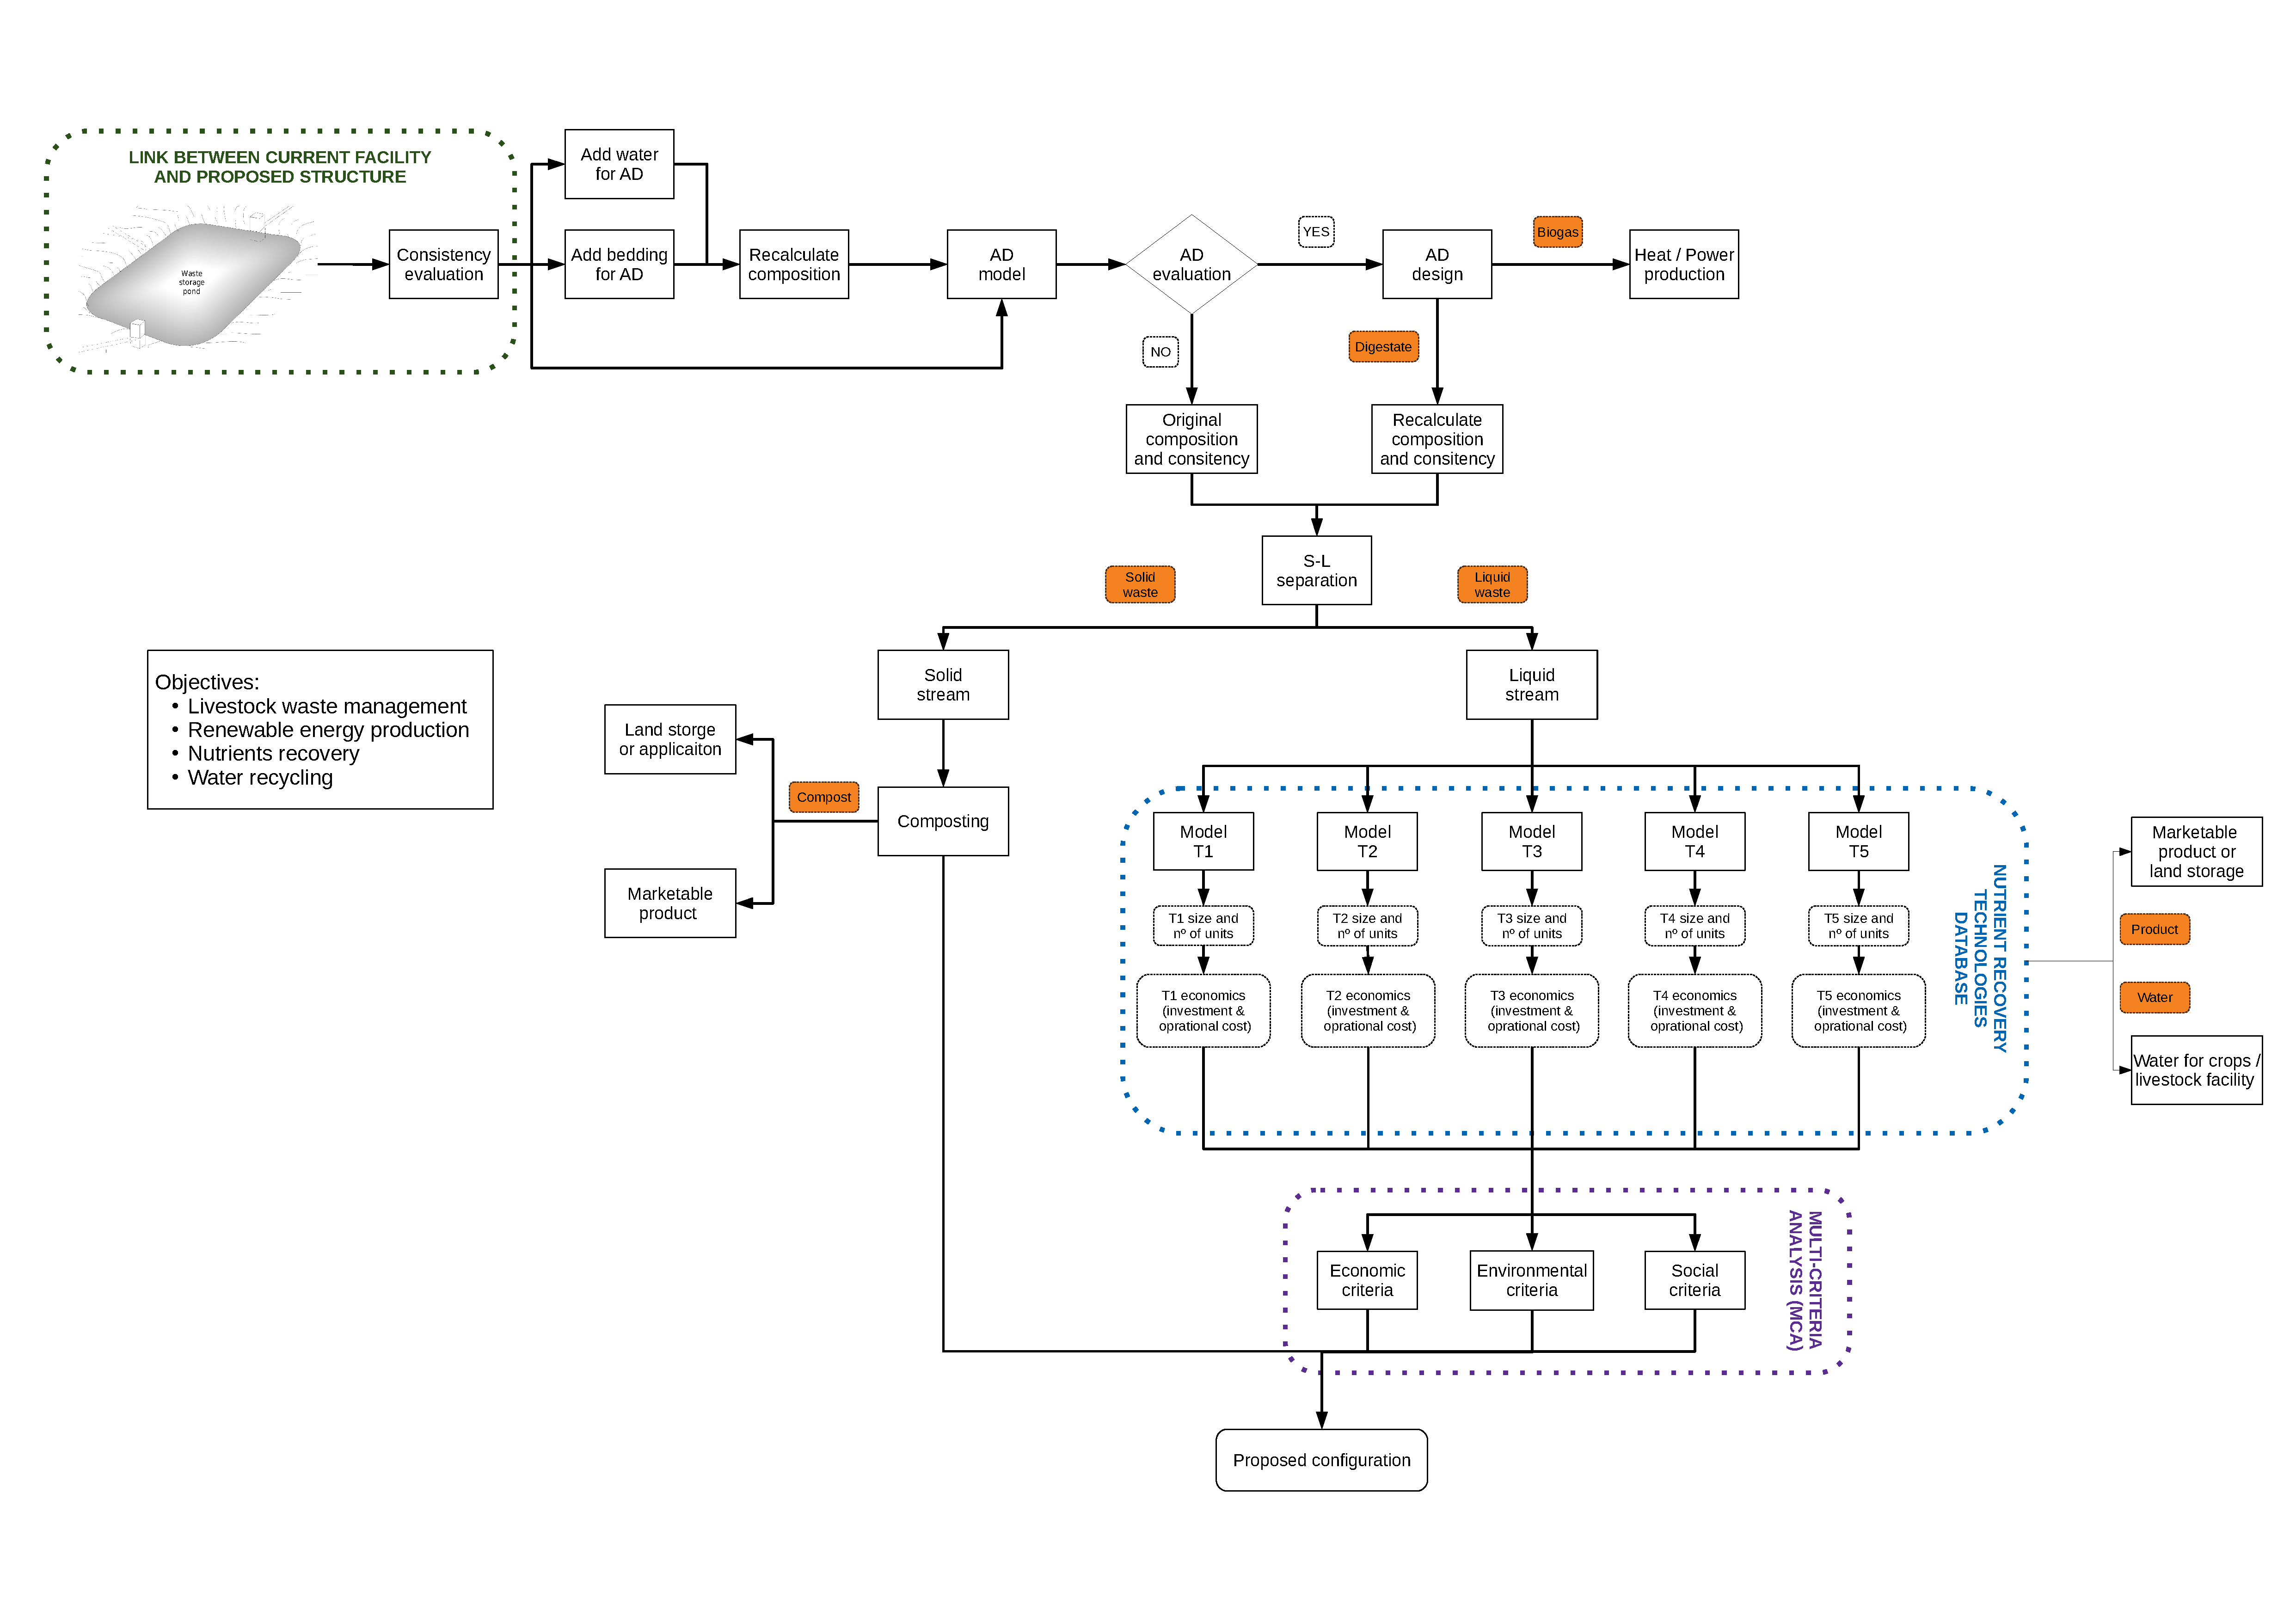
\includegraphics[width=\linewidth]{Process_Flowsheet} 
	\caption{Process flowsheet considered for manure treatment and nutrients recovery.}
	\label{fig:flowsheet}
\end{figure}

\section{Modularization and small scale}
Usually chemical facilities can be divided in two types:

\begin{itemize}
	\item \textbf{Monoproduct large scale continuous plants:} These facilities are very efficient in terms of energy and raw material utilization, but are inflexible because of their large size
	\item \textbf{Multiproduct batch plants:} These facilities are fleible, multiproduct capacity and have a quick response to the changes in the market. However as their are batch plants many times are inefficient from an energy and raw material utilization perspective.
\end{itemize}

To combine efficiency with flexibility at the same time, for the present work modular and small monoproduct plants which operate in continuous mode are proposed. On one hand, as they are small and modular the facilities are flexible, and can be located close to the waste generation places, which it is fundamental to reduce the transportation costs in cases where the localization of the raw material is geographically disperse, as the case of livestock residues. On the other hand as these plants operated in a monoproduct continuous mode they can achieve better efficiency than traditional batch plants.

The use of compatible modules is proposed with the aim of that the same design could be used for different processes (e.g. residues from different animals), which both design and possible sizes are standardized. \textbf{Therefore, the technical configuration of the facilities have to be made using a limited (discrete) number of possible modules and sizes.} As result of the use of discrete equipment sizes, the plants could operate within a determined range of operating conditions determined by the size of the different equipment. The optimization of the plant only could be optimized within the feasible range of operating conditions given by the size of the different equipment.

\section{Input data}
\subsection{Manure composition data}
HAY QUE ARREGLAR LOS DATOS DE ENTRADA DE MANURE PORQUE AHORA ESTA PARA DIGESTATE!

\section{Manure conditioning stage}
Currently, in the concentrated animal feeding operations (CAFOs), the manure is collected and stored as a liquid or slurry in waste storage ponds specifically designed for this purpose, or in tanks \cite{USDAHandbook}. However, if the anaerobic digestion (AD) stage will be implemented, following the recomendations of the U.S. Environmental Protection Agency, there exits a threshold regarding the total solids content in the manure 15\%, as shown in Fig. \ref{fig:TS_max} \cite{AgSTARHandbook}. If necessary, additional water should be added to reduce the solids content in manure before AD stage.

\begin{figure}[H]
	\centering
	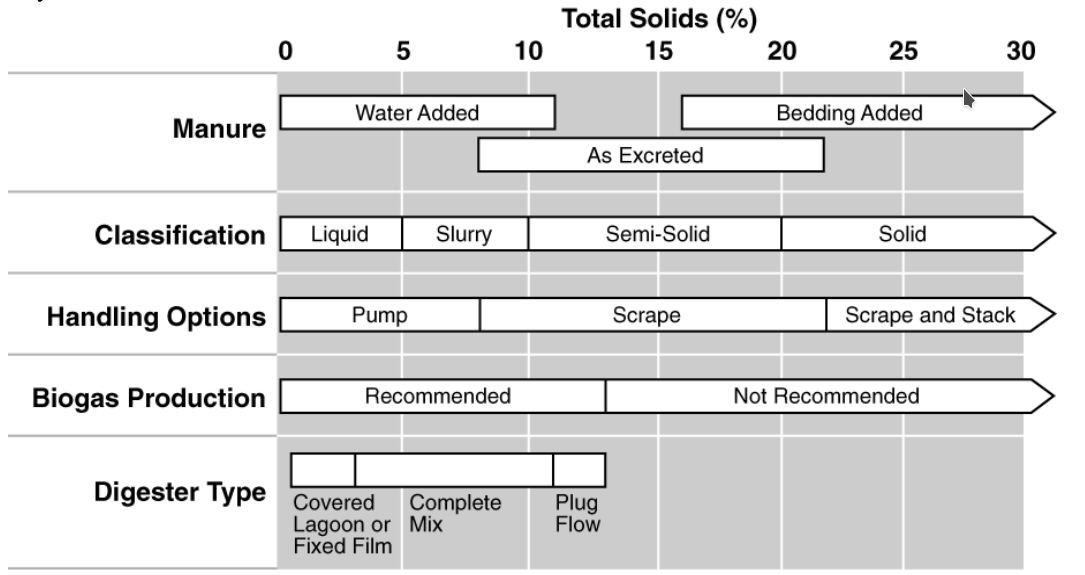
\includegraphics[width=0.6\linewidth]{TS_max} 
	\caption{Types of anaerobic digestion processes as function of the manure properties \cite{AgSTARHandbook}.}
	\label{fig:TS_max}
\end{figure}

PODRIAMOS AÑADIR EL TIPO DE BIORREACTOR MAS RECOMENDABLE EN LA APLICACIÓN TAMBIEN...PODEMOS PENSAR EN ELLO

\section{Anaerobic digestion stage}
AD is a complex microbiological process that decomposes organic matter in the absence of oxygen. It produces a gas mixture following hydrolysis, acidogenesis, acetogenesis, and methanogenesis steps, consisting mainly of methane and carbon dioxide (biogas), and decomposed substrate (digestate). The anaerobic reactor is modeled using mass balances of the species involved in the production of biogas and digestate. We refer the reader to \cite{Leon} for details on the modeling of the digester.

To estimate the cost of the digester units, a liner correlation between the investment cost and the animal population of the livestock facility has been developed from data reported by the U.S. Environmental Protection Agency (EPA) AgSTAR program \cite{AgSTAR2003}, shown in Fig. \ref{fig:AD_size_cost}
\begin{figure}[H]
	\centering
	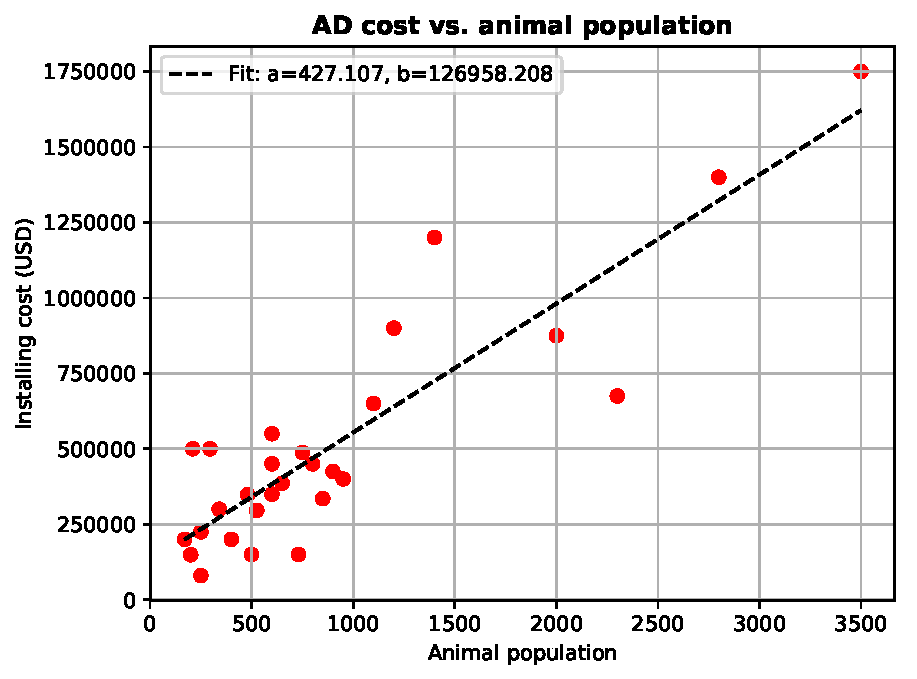
\includegraphics[width=0.6\linewidth]{AD_size_cost} 
	\caption{Correlation between AD units investment cost and animal population}
	\label{fig:AD_size_cost}
\end{figure}

The annual operation and management (O\&M) costs as function of the animal population are calculated as a fraction of the digester costs using a sigmoidal correlation developed from data reported by the U.S. Department of Agriculture (USDA) \cite{USDA_OM}, as shown in Fig. \ref{fig:AD_size_OM_Unit_cost}. It should be noted that O\&M costs do not include the capital cost amortization. Therefore, to estimate the total production cost the annualized equipment cost has been added to O\&M Costs, Eq.  \ref{eq:OM_inv_costs}. The plant lifetime assumed is 20 years. REVISAR ESTA ECUACION....AMORTIZACION?.

\begin{align} \label{eq:OM_inv_costs}
& \text{Operation cost} = \text{O\&M costs} + \frac{\text{Investment cost}}{\text{Plant lifetime}} 
\end{align}

\begin{figure}[H]
	\centering
	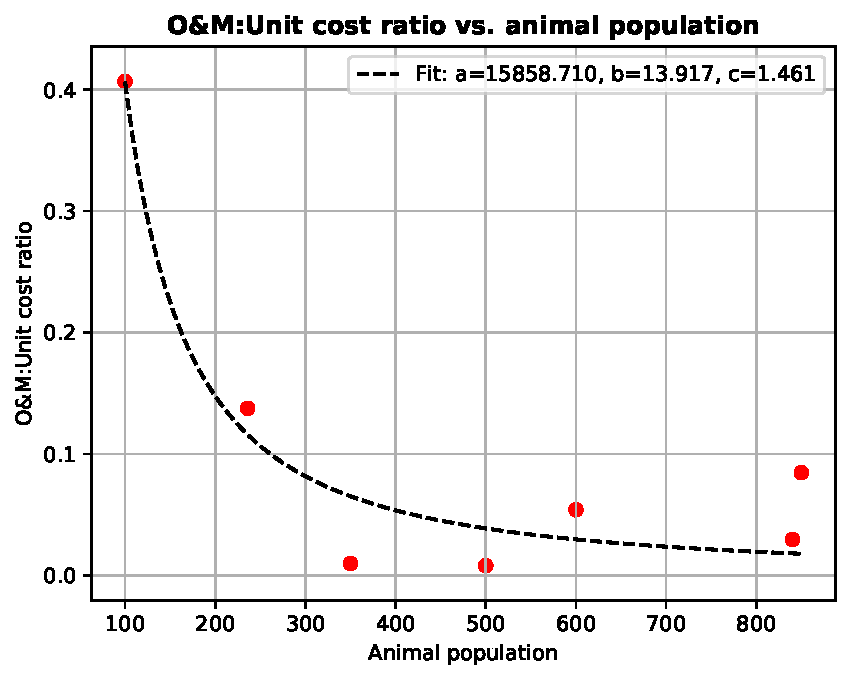
\includegraphics[width=0.6\linewidth]{AD_size_OM_Unit_cost} 
	\caption{Correlation between  O\&M:AD costs and livestock animal population}
	\label{fig:AD_size_OM_Unit_cost}
\end{figure}



Finally, due to the digestion process part of the organic nutrient are transformed in their inorganic forms. To evaluate the additional amount of P and N transformed from their organic forms to inorganic P and N, NH4:TKN diff and PO4:TP diff respectively, a statistical study from data available in literature was carried out. The results are shown in Table \ref{table:nut_mod}
%\begin{sidewaystable}%[H] 
	%	\begin{adjustwidth}{-1.6cm}{}
\begin{table}[H] 
	\centering
	\caption{Statistical summary of nutrients composition for cattle manure. Data from \cite{ADAS,Martin2,delaFuente,Sorensen}.} \label{table:nut_mod}
\begin{tabular}{ccccccccc}
	\toprule
	{} 	  &  TKN In		 &  TKN Out 	&  NH4 In 			&  NH4 Out 				&  TP In &			  TP Out &  			PO4 In &  				PO4 Out    \\
	\midrule
	count &    10.00 &        10.0 &     10.00 &                10.00 &                5.00 &                5.00 &                 5.00 &                 5.00    \\      
	mean  &   3856.10 &      3967.1 &  1845.90 &              2340.10 &             1442.60 &             1449.60 &               811.40 &               946.40    \\      
	std   &   847.41 &       942.9 &    354.59 &               387.34 &              467.14 &              485.29 &               277.67 &               331.88    \\      
	min   &   2920.00 &     2800.0 &    1300.00 &              1810.00 &              813.00 &              838.00 &               457.00 &               562.00   \\    
	25\%   &  3050.00 &     3152.5 &    1607.50 &              2047.50 &             1170.00 &             1170.00 &               590.00 &               670.00   \\  
	50\%   & 3660.00 &     3855.0 &     1825.00 &              2340.00 &             1450.00 &             1360.00 &               880.00 &               950.00   \\
	75\%   & 4630.75 &      4882.5 &    2159.75 &              2590.00 &             1860.00 &             1920.00 &              1050.00 &              1260.00   \\
	max   &     4960.00 &   5290.0 &     2300.00 &              2881.00 &             1920.00 &             1960.00 &              1080.00 &              1290.00  \\
	\bottomrule
\end{tabular}
\end{table}

%\end{sidewaystable}
\begin{table}[H] 
\centering
\begin{tabular}{ccccccc}
%	\centering
%	\caption{Statistical summary of nutrients composition for cattle manure $\left(\text{mg/L}\right)$. Data from \cite{Alburquerque,Bolzonella,Seppala,Gell,Normak,Sorensen,Tampere,Moset,Zheng,Xia,Moller,WRAP,ADAS,Risgberg,Ledda,Kirchmann,Moller2,Walsh,Loes,Martin2}.} \label{table:dig_compt_stats}
	\toprule
	{} &  NH4:TKN In &  		NH4:TKN Out &  		PO4:TP In &  	   PO4:TP Out &  NH4:TKN diff &  PO4:TP diff\\
	\midrule
		count&  	      10.00 &             10.00 &             5.00 &             5.00 &         10.00 &         5.00 \\
		mean&       0.48 &              0.60 &             0.56 &             0.65 &          0.24 &         0.16 \\
		std&        0.06 &              0.08 &             0.04 &             0.05 &          0.07 &         0.03 \\
		min&          0.39 &              0.48 &             0.50 &             0.57 &          0.17 &         0.14 \\
		25\%  &        0.47 &              0.56 &             0.56 &             0.64 &          0.21 &         0.14 \\
		50\% &         0.48 &              0.61 &             0.56 &             0.67 &          0.24 &         0.15 \\
		75\%&        0.53 &              0.66 &             0.56 &             0.67 &          0.27 &         0.19 \\
		max&         0.57 &              0.75 &             0.61 &             0.70 &          0.41 &         0.19 \\
	\bottomrule
\end{tabular}
\end{table}

CRITERIOS DE DECISION PARA ACEPTAR O NO AD?


\section{Solid-liquid separation stage}
Screw press is the technology selected based on the evaluation reported by M{\o}ller et al. \cite{MollerSLsep}. The experimental results reported in this work are used to determine the partition coefficients for the different elements, Table \ref{table:part_coef}.

\begin{table}[H] 
	\begin{adjustwidth}{}{}
		\centering
		\caption{Partition coefficients for solid-liquid manure separation using a screw press unit \cite{MollerSLsep}} \label{table:part_coef}
		\begin{tabular}{c c c}
			\toprule
%			\multicolumn{1}{c}{Number of units } &\multicolumn{4}{c}{Electrical power (kW)}\\
%			\cmidrule(lr){2-5}
			Element 	& Solid fraction & Liquid fraction	\\ \midrule
			Total mass 	& 0.08		& 0.92 \\
			Dry matter 	& 0.3054	& 0.6946 \\
			Org. N 		& 0.0938	& 0.9062 \\
			Org. P		& 0.2226 	& 0.7774 \\
		\end{tabular}
	\end{adjustwidth}
\end{table}

%A design correlation to relate the equipment sizing with the treated flow is developed AÑADIR REFERENCIA, Fig. \ref{fig:screwpress_size}. 
To determine the commercial sizes and number of units necessary as function of the flow to be treated, data from the manufacturer PWTech is considered \cite{PWTech}. Based on these data, the possible configurations in funciton of the flow are the following, Table \ref{table:ScrewPress_units}:

\begin{table}[H] 
	\begin{adjustwidth}{}{}
		\centering
		\caption{Sizing estimated for screw press units based on data from PWTech \cite{PWTech}} \label{table:ScrewPress_units}
		\begin{tabular}{c c c c c}
			\toprule
			\multicolumn{1}{c}{Load capacity $\left(\frac{m^{3}}{day}\right)$}&\multicolumn{4}{c}{Number of units}\\
			\cmidrule(lr){2-5}
			&\diameter(m) 0.23 & \diameter(m) 0.35 & \diameter(m) 0.42 & \diameter(m) 0.56	\\ \midrule
			$<$ 43 		& \cellcolor{blue!25}1 	& - 					& - & -	\\
			43 - 81 	& -						& \cellcolor{blue!25}1 	& - & - 	\\
			81 - 190 	& -						& - 					& \cellcolor{blue!25}1 & - 	\\
			190 - 381 	& -						& -					 	& \cellcolor{blue!25}2 & -	\\ 
			381 - 572 & -						& -					 	& \cellcolor{blue!25}3 & - 	\\ 
			572 - 708 & -						& -					 	& - & \cellcolor{blue!25}2	 	\\ 
			708 - 1090 & -						& -					 	& - & \cellcolor{blue!25}3	 	\\
			1090 - 1444 & -						& \-				 	& - & \cellcolor{blue!25}4	 	\\
			$>$ 1444 	&-						& -					 	& - & \cellcolor{blue!25}$\ceil[\bigg]{\frac{\text{Flow } \left(\sfrac{m^{3}}{day}\right)}{\text{Load Capacity}_{\text{\diameter 0.56m unit}}}}$  	\\
		\end{tabular}
	\end{adjustwidth}
\end{table}

The unit cost is based on the date reported by Matches \cite{Matches} for this type of equipment, as shown in Fig. \ref{fig:screwpress_investment_costs}. On the other hand, operating costs are calculated assuming the electrical power reported by the manufacturer for each model, as shown in Table \ref{table:ScrewPress_power} respectively.

%\begin{figure}[H]
%	\centering
%	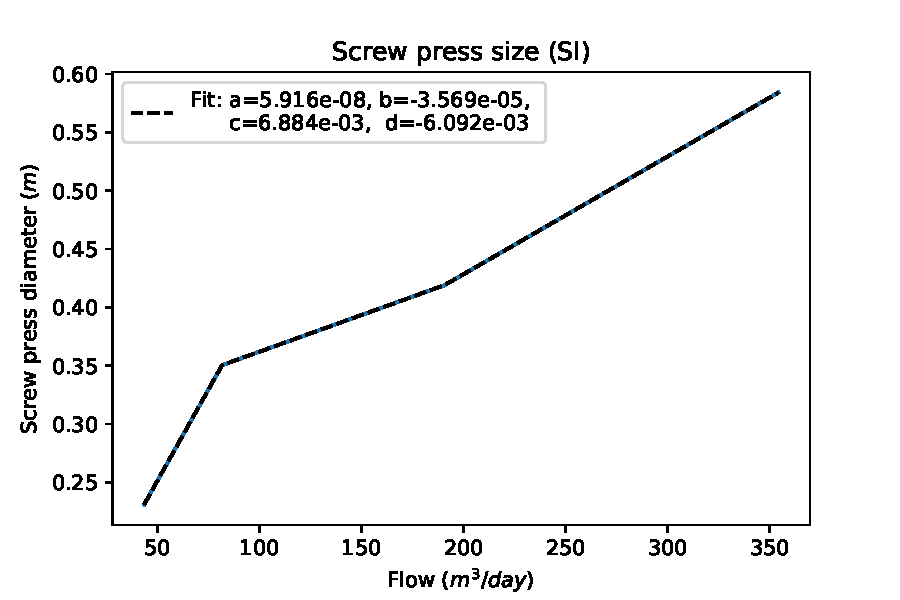
\includegraphics[width=0.6\linewidth]{screwpress_size_m} 
%	\caption{Sizing correlation relating screw press diameter and inlet flow.}
%	\label{fig:screwpress_size}
%\end{figure}

\begin{figure}[H]
	\centering
%	\begin{subfigure}[t]{0.5\linewidth}
	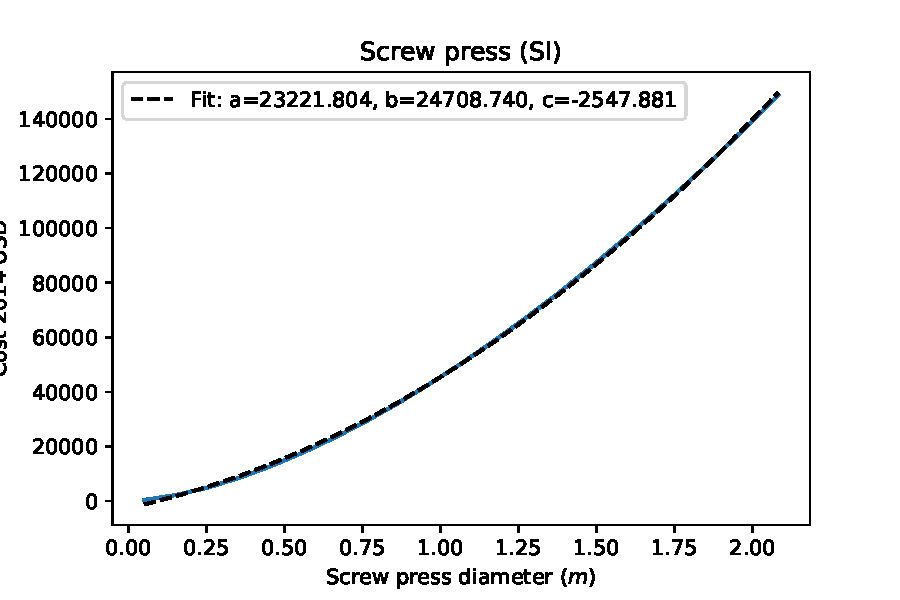
\includegraphics[width=0.6\linewidth]{screwpress_cost_m} 
	\caption{Estimated investment costs for solid-liquid separation using screw press units.}
	\label{fig:screwpress_investment_costs}
%	\end{subfigure}
%	\quad
%	\begin{subfigure}[t]{0.5\linewidth}
%		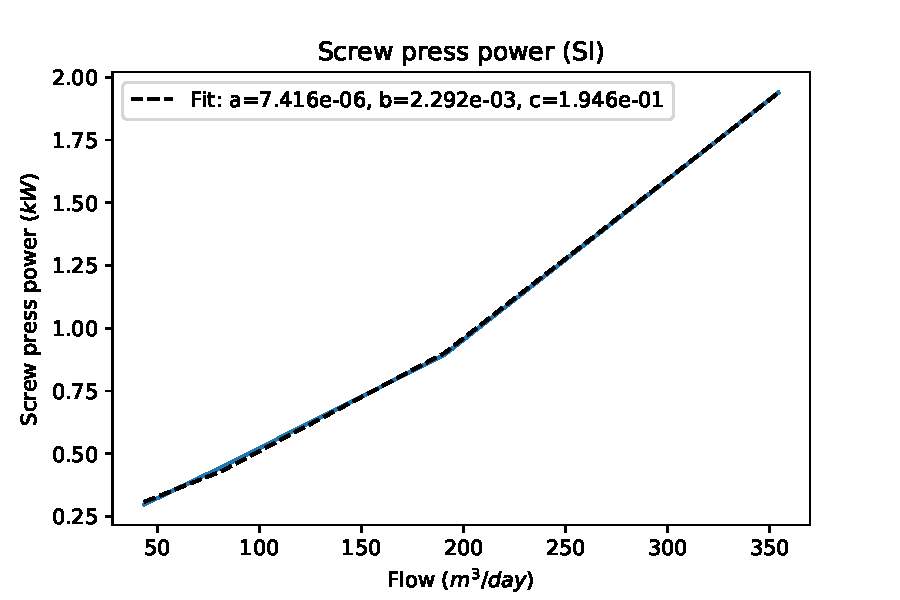
\includegraphics[width=\linewidth]{screwpress_power_kW}
%		\caption{Estimated operating costs for solid-liquid separation using screw press units.}
%		\label{fig:screwpress_operating_costs}
%	\end{subfigure}
%	
%	\caption{Estimated costs  for solid-liquid separation using screw press units.}
%	\label{fig:screwpress_costs}
\end{figure}

\begin{table}[H] 
	\begin{adjustwidth}{}{}
		\centering
		\caption{Electrical power of screw press units based on data from PWTech \cite{PWTech}} \label{table:ScrewPress_power}
		\begin{tabular}{c c c c c}
			\toprule
			\multicolumn{1}{c}{Number of units } &\multicolumn{4}{c}{Electrical power (kW)}\\
			\cmidrule(lr){2-5}
			&\diameter(m) 0.23 & \diameter(m) 0.35 & \diameter(m) 0.42 & \diameter(m) 0.56	\\ \midrule
			1 		& \cellcolor{blue!25}0.3 & \cellcolor{blue!25}0.45 & \cellcolor{blue!25}0.9 & -	\\
			2 	& -						& - 	& \cellcolor{blue!25}1.27 & \cellcolor{blue!25}3.88 	\\
			3	& -						& - 					& \cellcolor{blue!25}2.01 & \cellcolor{blue!25}6.34 	\\
			4 	& -						& - 					& - & \cellcolor{blue!25}7.83 \\
		\end{tabular}
	\end{adjustwidth}
\end{table}

Finally, assuming the units discretization considered in Table \ref{table:ScrewPress_units}, the investment and operating costs are presented in Figs \ref{fig:screwpress_unit_cost_m} and \ref{fig:screwpress_op_cost_m} respectively.
\begin{figure}[H]
	\begin{subfigure}[t]{0.5\linewidth}
		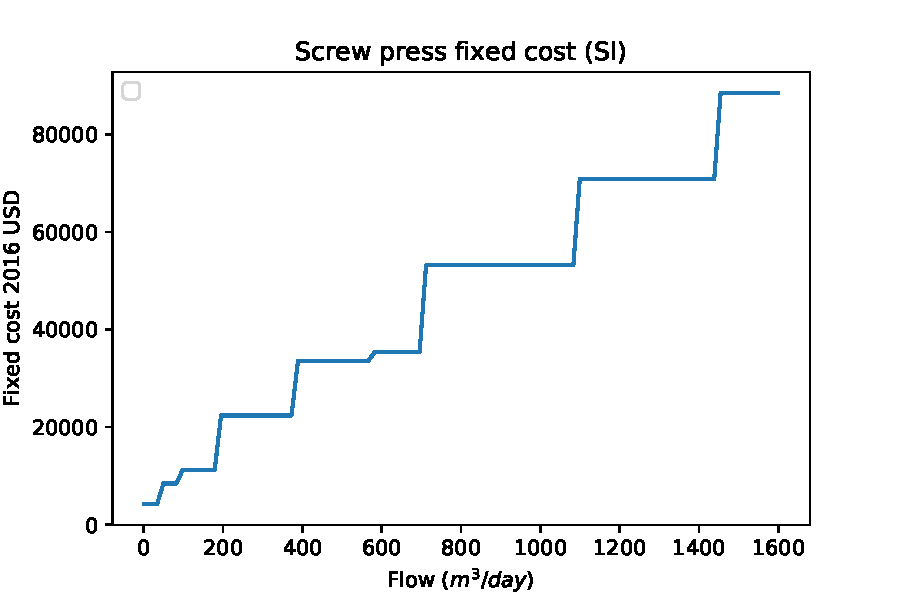
\includegraphics[width=\linewidth]{screwpress_unit_cost_m} 
		\caption{Estimated investment costs for screw press units.}
		\label{fig:screwpress_unit_cost_m}
	\end{subfigure}
	\quad
	\begin{subfigure}[t]{0.5\linewidth}
		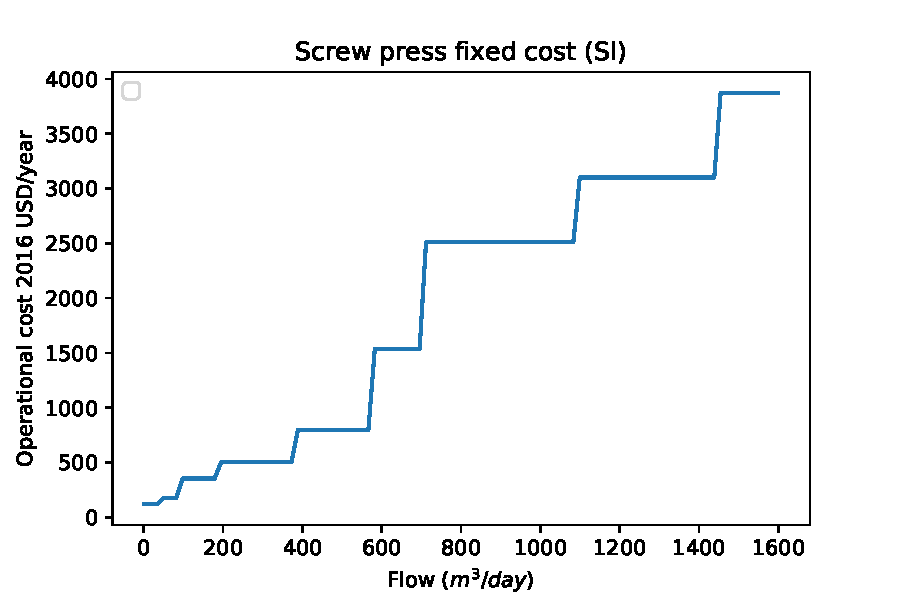
\includegraphics[width=\linewidth]{screwpress_op_cost_m}
		\caption{Estimated operation costs for screw press units.}
		\label{fig:screwpress_op_cost_m}
	\end{subfigure}
	
%	\caption{Estimated costs for screw press units.}
	\label{fig:screwpress_costs}
\end{figure}


\section{Nutrient recovery technologies}
\subsection{Base case: composting}
Composting

\subsection{Filtration}
Package filters are considered for small facilities, while gravity filtration systems for larger flows, acording with the recomendations reported by the U.S. Environmental Agency (EPA) \cite{EPAWWTPCosts_V2, EPAWWTPCosts_V3}. The flow ranges for each filter size, filter type, and number of units are shown in Table \ref{table:Filter_units}.

\begin{table}[H] 
	\begin{adjustwidth}{}{}
		\centering
		\caption{Flow ranges, filter type, and number of units for filtration processes \cite{EPAWWTPCosts_V2, EPAWWTPCosts_V3}} \label{table:Filter_units}
		\begin{tabular}{c c c }
			\toprule
			\multicolumn{1}{c}{Load capacity $\left(\frac{m^{3}}{hr}\right)$}&\multicolumn{2}{c}{Number of units}\\
			\cmidrule(lr){2-3}
			&Pressure filter & Gravity filter 	\\ \midrule
			$<$ 0.16 		& \cellcolor{blue!25}1 		& - 	\\
			0.16 - 0.39 	& \cellcolor{blue!25}1		& - 	\\
			0.39 - 1.59 	& \cellcolor{blue!25}1		& - 	\\
			1.59 - 3.86 	& \cellcolor{blue!25}1		& -		\\ 
			3.86 - 6.36 	& \cellcolor{blue!25}1		& -		\\ 
			6.36 - 18.17 	& \cellcolor{blue!25}1		& -	 	\\ 
			18.17 - 38.61 	& -							& \cellcolor{blue!25}2	\\
			38.61 - 65.30   & -							& \cellcolor{blue!25}2 	\\
			65.30 - 95.39  	& -							& \cellcolor{blue!25}2 	\\
			95.39 - 143.09  & -							& \cellcolor{blue!25}2 	\\
			143.09 - 317.97 & -							& \cellcolor{blue!25}2 	\\
		\end{tabular}
	\end{adjustwidth}
\end{table}

Additionaly, the investment and operating costs reported by the EPA for theses sizes are shown in Figs. \ref{fig:filter_investment_costs} and \ref{fig:filter_operating_costs} respectively \cite{EPAWWTPCosts_V2, EPAWWTPCosts_V3}.
\begin{figure}[H]
	\begin{subfigure}[t]{0.5\linewidth}
		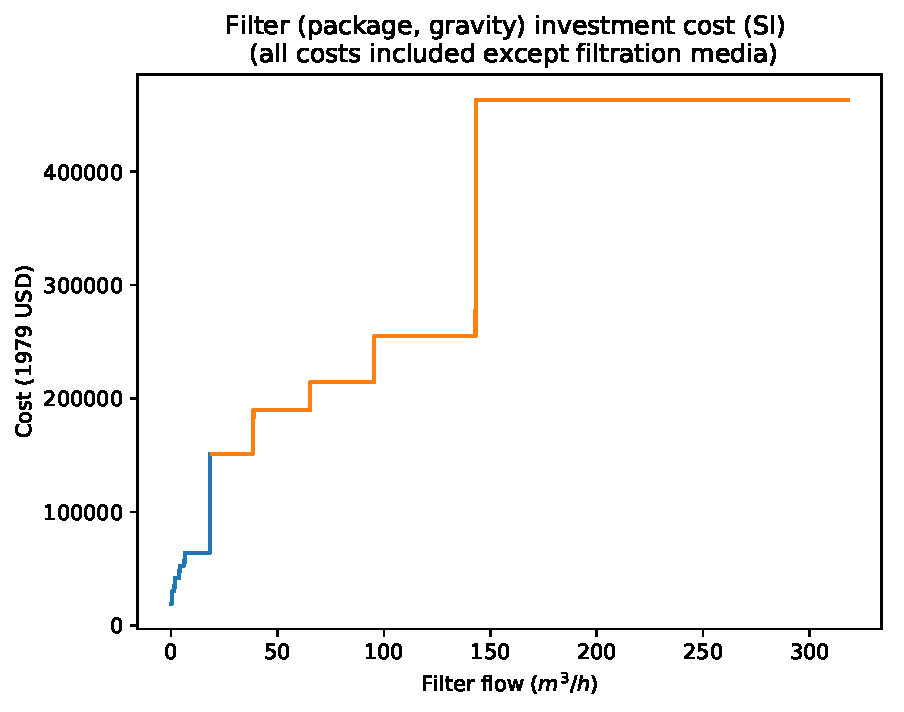
\includegraphics[width=\linewidth]{filter_pressure_gravity_investment_cost_m} 
		\caption{Estimated investment costs for filtration processing.}
		\label{fig:filter_investment_costs}
	\end{subfigure}
	\quad
	\begin{subfigure}[t]{0.5\linewidth}
		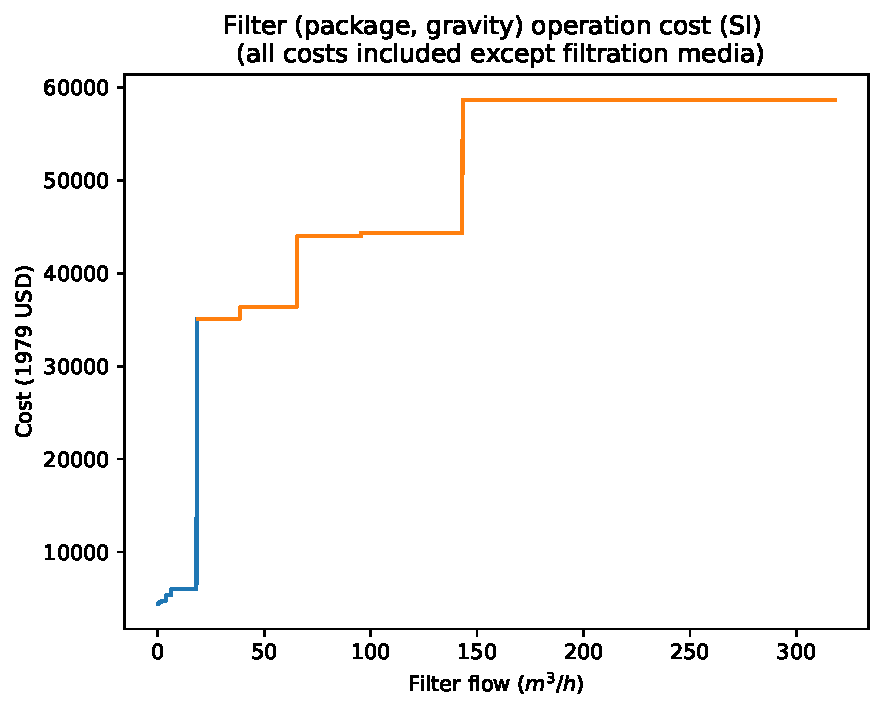
\includegraphics[width=\linewidth]{filter_pressure_gravity_operation_cost_m}
		\caption{Estimated operation costs for filtration processing.}
		\label{fig:filter_operating_costs}
	\end{subfigure}
	
	\caption{Estimated costs for filtration processing \cite{EPAWWTPCosts_V2, EPAWWTPCosts_V3}.}
	\label{fig:filtration_costs}
\end{figure}

\subsection{Low quality struvite produciton}
Struvite production in CSTR reactor. This process is formed by 3 stages: the struvite formation in a CSTR reactor, the separation of the struvite from the liquid phase using a clarifier step followed by a filtration step in a vacuum conveyor unit, and finally a drying stage in a conveyor dryer.

\subsubsection{CSTR reactor}
The estimation of the investment CSTR reactor unit is the result of the sum of the vessel and the agitator costs. For design purposes, a maximum CSTR volume of 45 m\textsuperscript{3} is considered \cite{CAPCOST}. For larger volumes, multiple units installed in parallel are considered, Eq. \ref{eq:CSTR_units}.

\begin{align} \label{eq:CSTR_units}
& \text{Number of CSTR} = \ceil[\bigg]{\frac{\text{Total volume }}{\text{Max. sixe}}}
\end{align}

The vessel cost is based on data reported by CAPCOST \cite{CAPCOST}, from which the correlation shown in Fig. \ref{fig:vessel_investment_cost} has been developed.
\begin{figure}[H]
	\centering
	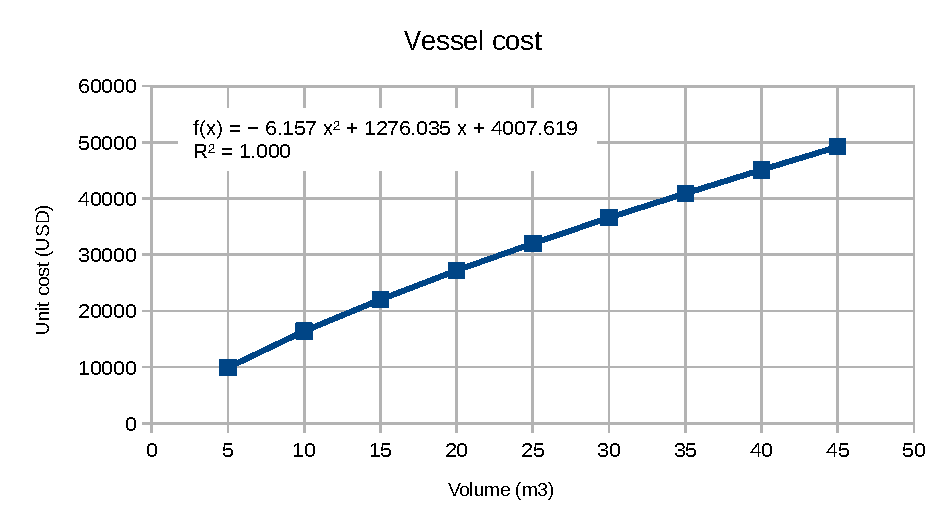
\includegraphics[width=0.6\linewidth]{vessel_investment_cost} 
	\caption{Estimated investment costs for a non-jacketed vessel, based on data from CAPCOST \cite{CAPCOST}.}
	\label{fig:vessel_investment_cost}
\end{figure}

Unit and operation costs operation of the agitator are based on the correlations reported in Couper et al. \cite{Walas}, Eqs. \ref{eq:agitator_cost} and \ref{eq:agitator_op_cost} respectively. This correlation is based in the power of the agitator, estimated using Eq. \ref{eq:agitator_power} , where the $Power_{specefic}$ for slurries is equal to 10 HP per 1000 gal \cite{Walas}.

\begin{align} 
& \text{Power}_{\text{agitator}} \ \left(HP\right) =  V\left(US \ gallon\right) \cdot\frac{Power_{specefic}}{1000} \label{eq:agitator_power} \\
& \text{Agitator cost} \ \left(2009 \ USD\right) = 1.218 \cdot exp[9.25 + 0.2801  \cdot ln(Power_{agitator})+0.0542 \cdot (ln(Power_{agitator}))^2] \label{eq:agitator_cost}\\
& \text{Agitator operation cost}  = Power_{agitator}\left(kW\right) \cdot Electricity_{price} \cdot 3600 \cdot 24 \cdot 365 \cdot 3600^{-1} \label{eq:agitator_op_cost}
\end{align}

\subsubsection{Clarifier}
The clarifier cost has been estimated as a vessel, using the correlation shown in Fig. \ref{fig:vessel_investment_cost}. The residence time assumed is 1 hour. JUSTIFICAR ESTO

\subsubsection{Vacuum conveyor filter}
Vacuum converyor filter has been selected due to this features makes it an adequate alternative for struvite recovery. Additionally, this technology it has been used in some previous studies \cite{Matynia}. For design purposes, a filter rate of 0.011 kg/(m\textsuperscript{2}·s) and a maximum area of 1200 ft\textsuperscript{2} are considered \cite{Walas}. Unit cost is based on the correlations reported in Couper et al. \cite{Walas}, Eq. \ref{eq:beltfilter_cost}. This correlation is based in the area of the filter, estimated using Eq. \ref{eq:beltfilter_area}.

\begin{align} 
& \text{\text{Area}}_{\text{filter}} \ \left(m^{2}\right) = \frac{Flow \left( \frac{kg}{s} \right)}{Rate_{filtration} \left( \frac{kg}{m^{2} \cdot s} \right)} \label{eq:beltfilter_area} \\
& \text{Filter cost} \ \left(2009 \ USD\right) = \frac{45506}{Area_{filter}^{0.5} \left( ft^{2} \right)} \cdot Area_{filter} \left( ft^{2} \right) \label{eq:beltfilter_cost}
\end{align}


\subsubsection{Drying stage in a conveyor dryer unit}
The final drying of struvite is made with a conveyor dryer.For design purposes, a drying time of 2100 s and a dryer capacity of 20.85 kg/m\textsuperscript{2} are assumed based on data reported on Table 12-21 of the Perry's book \cite{Perry}. The dryer loading and dryer area are estimated using Eqs. \ref{eq:dryer_loading} and \ref{eq:dryer_area}, respectively.

\begin{align} 
& \text{\text{Loading}}_{\text{dryer}} \ \left(kg\right) = Flow \left( \frac{kg}{s} \right) \cdot time_{drying} \left( s\right) \label{eq:dryer_loading} \\
& \text{\text{Area}}_{\text{dryer}} \ \left(m^2\right) = \frac{Loading_{dryer}\left(kg\right)}{Capacity_{dryer} \left(\frac{kg}{m^2}\right)} \label{eq:dryer_area}
\end{align}

The cost estimation for a conveyor unit is based on data reported in Table 12-23 of the Perry's book \cite{Perry}. The correlation developed, relating the unit cost and its area can be found in Fig. \ref{fig:converyor_dryer_investment_cost}. Additionaly, based on these data, a maximun conveyor dryer size of 90 m\textsuperscript{2} is assumed.
\begin{figure}[H]
	\centering
	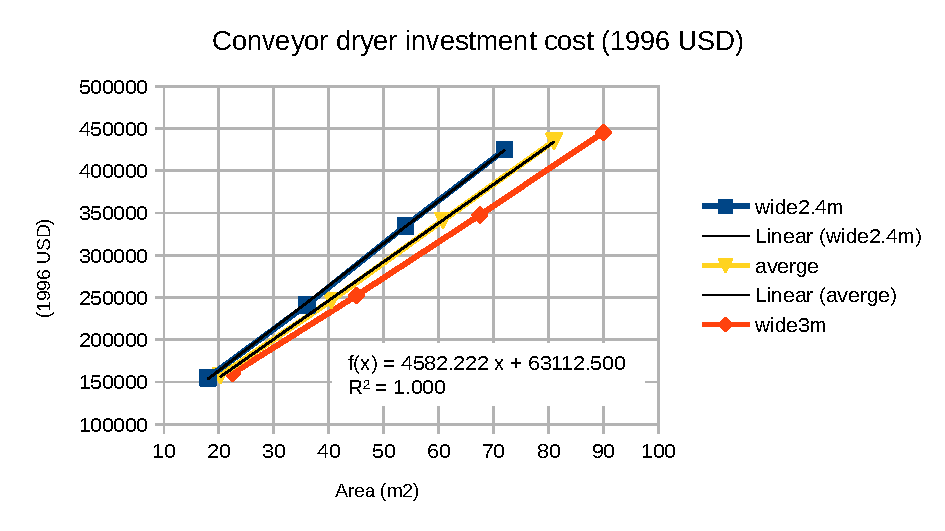
\includegraphics[width=0.6\linewidth]{converyor_dryer_investment_cost} 
	\caption{Estimated investment costs for conveyor dryer unit.}
	\label{fig:converyor_dryer_investment_cost}
\end{figure}

The operation cost of this unit is estimated in basis on natural gas neccesary to evaporate the water content in the stream, Eqs. \ref{eq:latent_heat} to \ref{eq:_costnat_gas}.

\begin{align} 
& \text{\text{Q}}_{\text{latent}} \ \left(\frac{kJ}{s}\right) = Flow_{water} \left( \frac{kg}{s} \right) \cdot \lambda_{water} \left( \frac{kJ}{kg}\right) \label{eq:latent_heat} \\
& \text{\text{V}}_{\text{natural gas}} \ \left(\frac{m^3}{s}\right) = \frac{Q_{latent}}{\lambda_{natural \ gas}\left( \frac{kJ}{m^3}\right) \cdot efficiency} \label{eq:nat_gas} \\
& \text{\text{Operating cost}}_{\text{dryer}} \ \left(\frac{USD}{year}\right) = V_{natural \ gas} \cdot Price_{natural \ gas} \cdot 3600 \cdot 24 \cdot 365 \label{eq:_costnat_gas} \\
\end{align}

\subsection{High quality struvite produciton}
Nutrient recovery trough the formaiton of strivite has been widely described in literature, mainly focused in phosphorus recovery. However, usually the experimental data available to evaluated the efficiency and feasibility of P recovery through struvite formation are developed for municipal wastewater. Therfore, specific correlations for livestock wastewater to estimate the molar fraction of $\left(PO_{4}^{3-}\right)$ and $\left(Ca^{2+}\right)$ recovered as precipitates, were developed from a thermodynamic perspective in previous work, \cite{MartinStruvite}, Eqs \ref{eq:sigmoidal_Ca_StrYield} to \ref{eq:sigmoidal_CaCaCO3}, where $ x_{Ca^{2+}:PO_{4}^{3-}}$ is referred to the $Ca^{2+}/PO_{4}^{3-} \ \text{molar ratio}$.
\begin{align}
&x_{struvite \left(PO_{4}^{3-}\right) }= \frac{0.798}{1+\left(x_{Ca^{2+}:PO_{4}^{3-}} \cdot 0.576\right)^{2.113}} \label{eq:sigmoidal_Ca_StrYield} \\
\nonumber \\
\begin{split}
& x_{hydroxyapatite \left(Ca^{2+}\right)} = -4.321 \cdot 10^{-2} \cdot x_{Ca^{2+}:PO_{4}^{3-}}^{2} + 0.313 \cdot x_{Ca^{2+}:PO_{4}^{3-}} \\& \hspace{7.8cm} - 3.619 \cdot 10^{-2} \label{eq:sigmoidal_Ca_HAP}
\end{split}
\\
\nonumber \\
&  x_{CaCO_{3} \left(Ca^{2+}\right)} = \frac{1.020}{1+\left(x_{Ca^{2+}:PO_{4}^{3-}} \cdot 0.410 \right)^{1.029}} \label{eq:sigmoidal_CaCaCO3}
\end{align}

These correlations are used in the model to calculate the mass flows of the precipitates formed, Eqs \ref{eq:fc_sigmoidal_Ca_StrYield} to \ref{eq:fc_sigmoidal_CaCaCO3}.

\begin{align}
&fc_{struvite} = \left(fc_{\left(PO_{4}^{3-}\right)} \cdot \frac{1}{MW_{P}} \cdot x_{struvite \left(PO_{4}^{3-}\right) } \cdot \frac{1 \ kmol_{struvite}}{1 \ kmol_{PO_{4}^{3-}}} \cdot MW_{struvite}\right) \cdot P_{SS} \label{eq:fc_sigmoidal_Ca_StrYield} \\
&fc_{hydroxyapatite} = \left(fc_{\left(Ca^{2+}\right)} \cdot \frac{1}{MW_{Ca}} \cdot x_{hydroxyapatite \left(Ca^{2+}\right)}  \cdot \frac{1 \ kmol_{hydroxyapatite}}{5 \ kmol_{Ca^{2+}}} \cdot MW_{hydroxyapatite} \right) \cdot P_{SS} \label{eq:fc_sigmoidal_Ca_HAP} \\
&fc_{CaCO_{3}} = \left(fc_{\left(Ca^{2+}\right)} \cdot \frac{1}{MW_{Ca}} \cdot x_{CaCO_{3} \left(Ca^{2+}\right)}  \cdot \frac{1 \ kmol_{CaCO_{3}}}{1 \ kmol_{Ca^{2+}}} \cdot MW_{CaCO_{3}} \right) \cdot P_{SS} \label{eq:fc_sigmoidal_CaCaCO3}
\end{align}

Where $P_{SS}$ is a penalization due to the presence of suspended solids in the medium, which has been developed as follows:

Struvite production in FBR reactor. Standard sizes and capacities are shown in Fig. \ref{fig:ostara_sizes}, while investment and operation costs can be found in Fig. \ref{fig:ostara_costs}\cite{Pearl500cost1,Pearl2Kcost1,Pearl2Kcost2, Pearl10Kcost1,Pearl10Kcost2}

\begin{figure}[H]
	\centering
	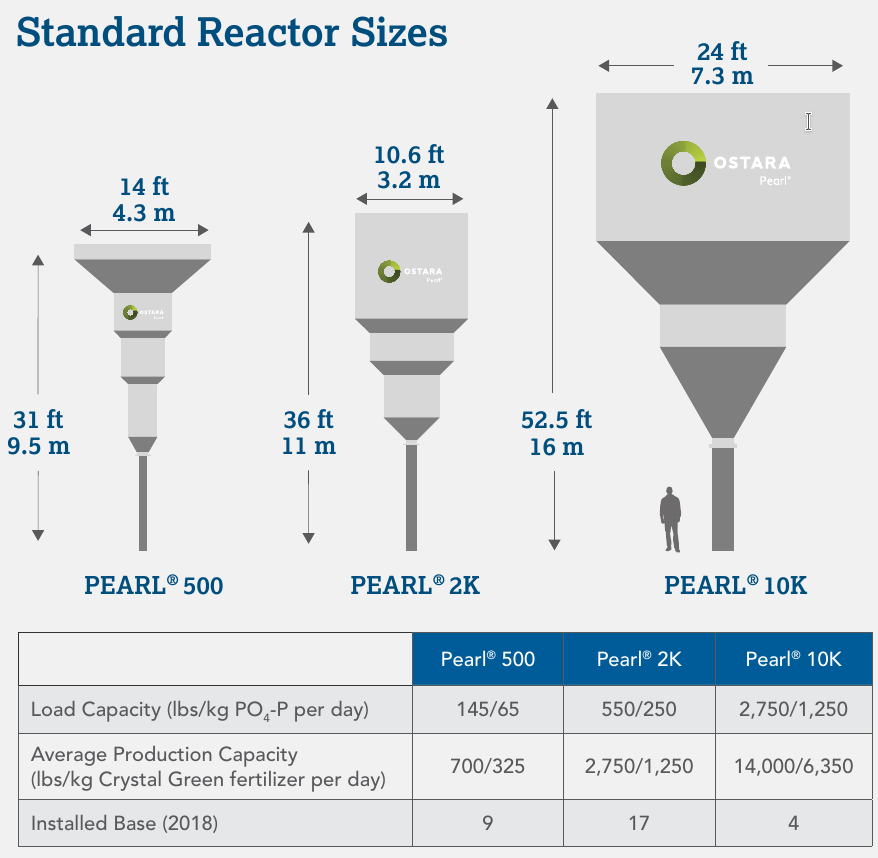
\includegraphics[width=0.6\linewidth]{ostara_sizes} 
	\caption{Standard sizes considered for struvite production using FBR reactor.}
	\label{fig:ostara_sizes}
\end{figure}

%\begin{figure}[H]
%	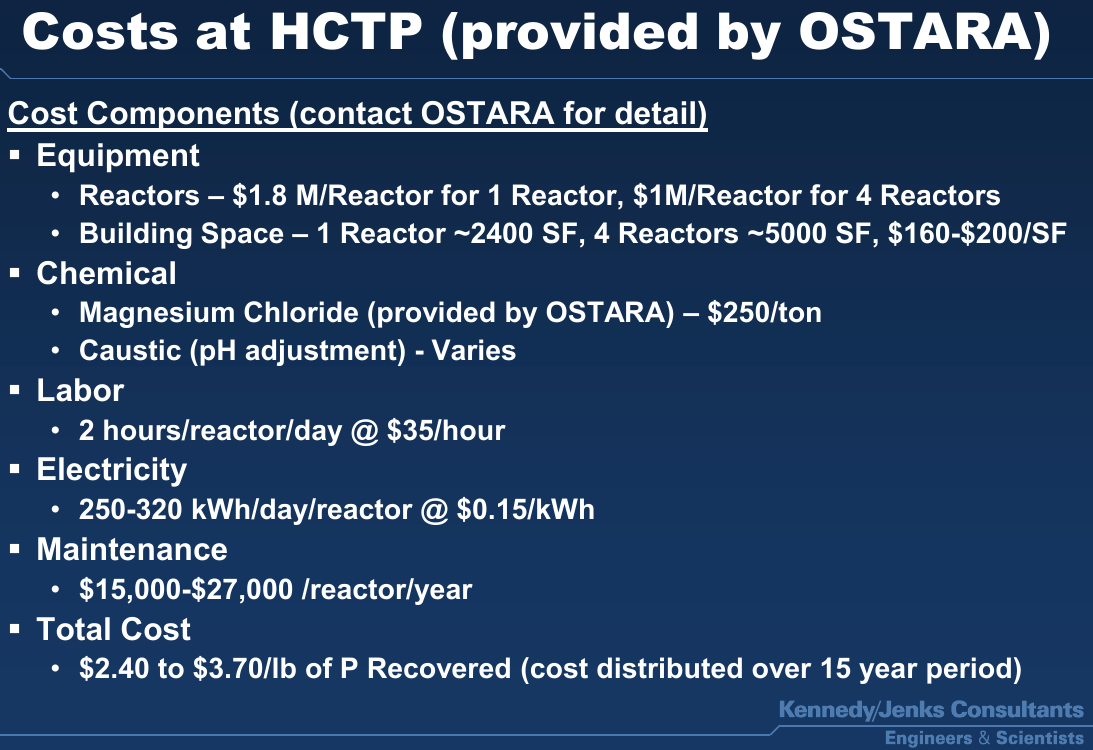
\includegraphics[width=\linewidth]{ostara_costs} 
%	\caption{Estimated costs for struvite production using FBR reactor.}
%	\label{fig:ostara_costs}
%\end{figure}

\begin{figure}[H]
	\begin{subfigure}[t]{0.5\linewidth}
		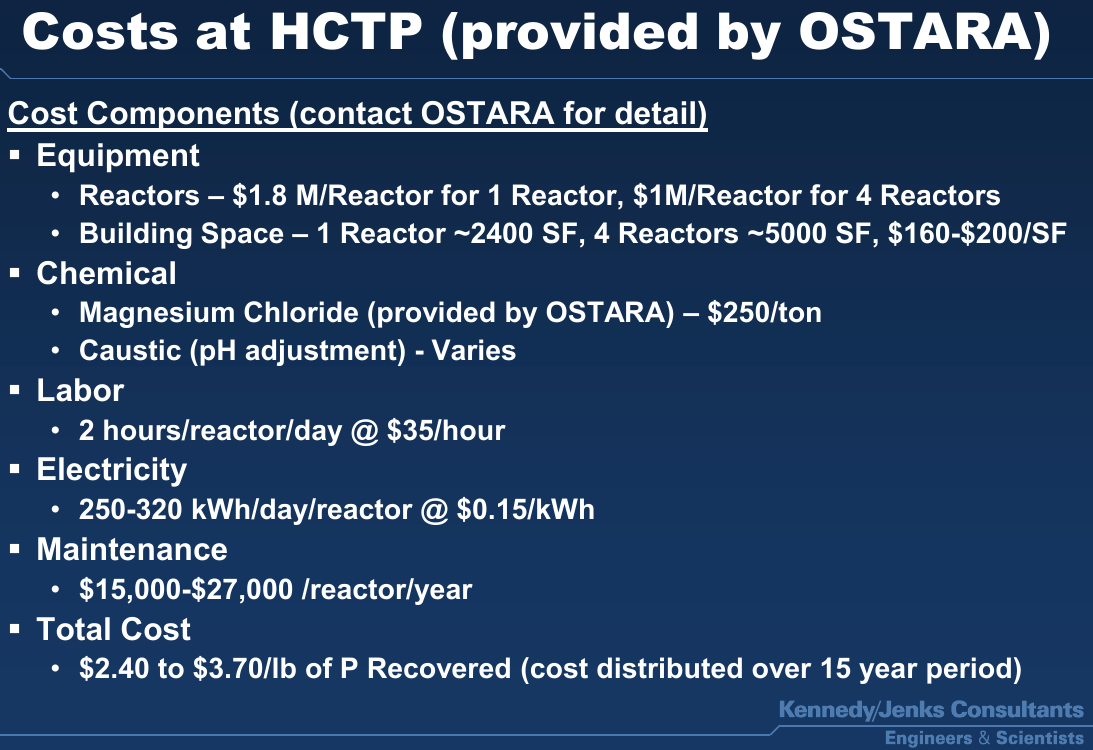
\includegraphics[width=\linewidth]{ostara_costs} 
%		\caption{Estimated costs for struvite production using FBR reactor.}
%		\label{fig:ostara_costs}
	\end{subfigure}
	\quad
	\begin{subfigure}[t]{0.5\linewidth}
		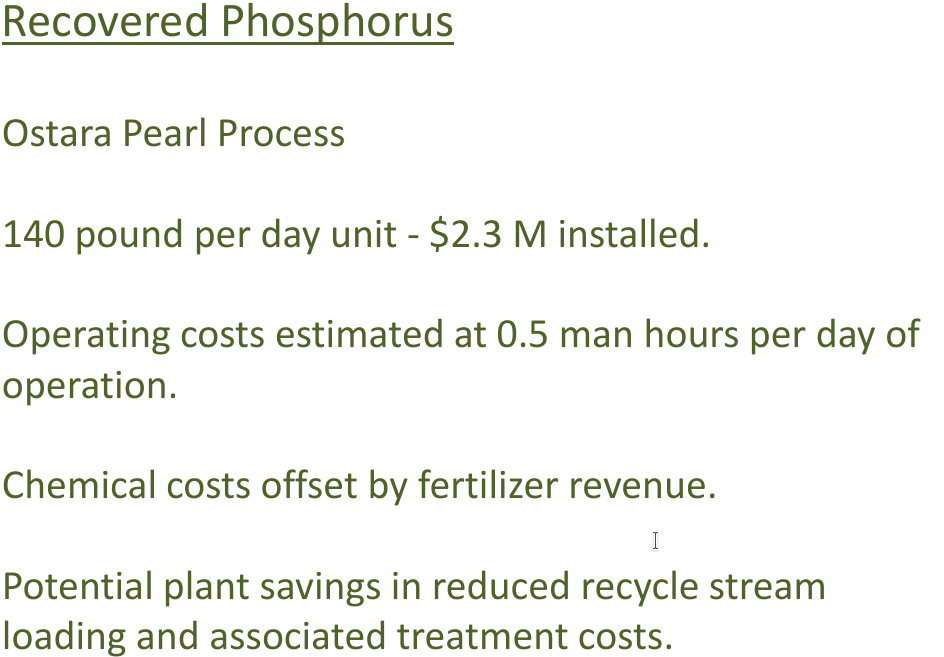
\includegraphics[width=\linewidth]{ostara_costs2}
%		\caption{Estimated costs for struvite production using FBR reactor.}
%		\label{fig:ostara_costs}
	\end{subfigure}
	
	\caption{Estimated costs for struvite production using FBR reactor.}
	\label{fig:ostara_costs}
\end{figure}

\begin{table}[H] 
	\begin{adjustwidth}{}{}
		\centering
		\caption{Sizing and equipment cost estimated for Ostara Pearl process} \label{table:ostara_costs}
		\begin{tabular}{c c c c}
			\toprule
			& Pearl\textsuperscript{\textregistered} 500 & Pearl\textsuperscript{\textregistered} 2K	& Pearl\textsuperscript{\textregistered} 10K	\\ \midrule
%			\cmidrule(lr){2-4}
			Load capacity $\left(\frac{\text{kg}_{\text{PO}_\text{4}}}{day}\right)$ & 65 & 250 & 1250 	\\ \\
			Equipment cost (USD)	& $2.3 \cdot 10^{6}$ & $3.1 \cdot 10^{6}$  & $10.0 \cdot 10^{6}$  	\\ \\
			Investment - $\frac{\text{kg}_{\text{PO}_\text{4}}}{day}$ ratio $\left(\frac{USD}{kg}\right)$	& 35385 & 12252 & 8000  \\ 
			\bottomrule 
		\end{tabular}
	\end{adjustwidth}
\end{table}

An investment cost - equipment cost ratio of 1.9 is derived from \cite{Pearl2Kcost2}.

Discrete equipment selection is assumed considering the criteria for sizing and determine the number of units necessary collected in Table \ref{table:ostara_units}, based on the information reported by Ostara \cite{Ostara}

\begin{table}[H] 
	\begin{adjustwidth}{}{}
		\centering
		\caption{Sizing and investment cost estimated for Ostara Pearl process} \label{table:ostara_units}
		\begin{tabular}{c c c c}
			\toprule
			\multicolumn{1}{c}{Load capacity $\left(\frac{\text{kg}_{\text{PO}_\text{4}}}{day}\right)$}&\multicolumn{3}{c}{Number of units}\\
			\cmidrule(lr){2-4}
			 & Pearl\textsuperscript{\textregistered} 500 & Pearl\textsuperscript{\textregistered} 2K	& Pearl\textsuperscript{\textregistered} 10K	\\ \midrule
			$<$ 65 		& \cellcolor{blue!25}1 	& - 					& - 	\\
			65 - 250 	& -						& \cellcolor{blue!25}1 	& -  	\\
			250 - 500 	& -						& \cellcolor{blue!25}2 	& -  	\\
			500 - 1250 	& -						& -					 	& \cellcolor{blue!25}1  	\\ 
			1250 - 1500 & -						& \cellcolor{blue!25}1 	& \cellcolor{blue!25}1  	\\ 
			1500 - 1750 & -						& \cellcolor{blue!25}2 	& \cellcolor{blue!25}1	 	\\ 
			$>$ 1750 	&-						& -					 	& \cellcolor{blue!25}$\ceil[\bigg]{\frac{\text{kg}_{\text{PO}_\text{4}} \text{ recovered}}{\text{Load Capacity}}}$  	\\
		\end{tabular}
	\end{adjustwidth}
\end{table}

The operation cost considered are chemicals, electricity and labor costs. The specific values assumed for these items are shown in Table \ref{table:ostara_op_costs} \cite{Pearl2Kcost2}.

\begin{table}[H] 
	\begin{adjustwidth}{}{}
		\centering
		\caption{Operation costs items for estiomation of the Ostara process operation costs} \label{table:ostara_op_costs}
		\begin{tabular}{c c}
			\toprule
			Item & Value \\ \midrule
			%			\cmidrule(lr){2-4}
			$\text{MgCl}_{2}$ dosing $\left(MgCl_{2}:PO_{4}^{3-} \text{ molar ratio} \right)$ & 2 \\
			Electricity demand $\left( \sfrac{kWh}{reactor \cdot day} \right)$	& 220 \\
			Labour $\left( \sfrac{hour}{reactor \cdot day} \right)$	& 2   \\ 
			Maintenance $\left( \sfrac{USD}{reactor \cdot year} \right)$	& 21000   \\
			\bottomrule 
		\end{tabular}
	\end{adjustwidth}
\end{table}

High quality struvite production using FBR reactors is formed by two stages: the struvite formation in a FBR reactor, and a drying stage in a conveyor dryer. However the conveyor dryer cost is already considered in the estimation shown in Table \ref{table:ostara_costs} \cite{Pearl2Kcost2}.

%\subsubsection{Drying stage in a conveyor dryer unit}
%The investment for a conveyor unit in based to its drying area can be found in Fig. \ref{fig:converyor_dryer_investment_cost2}
%\begin{figure}[H]
%	\centering
%	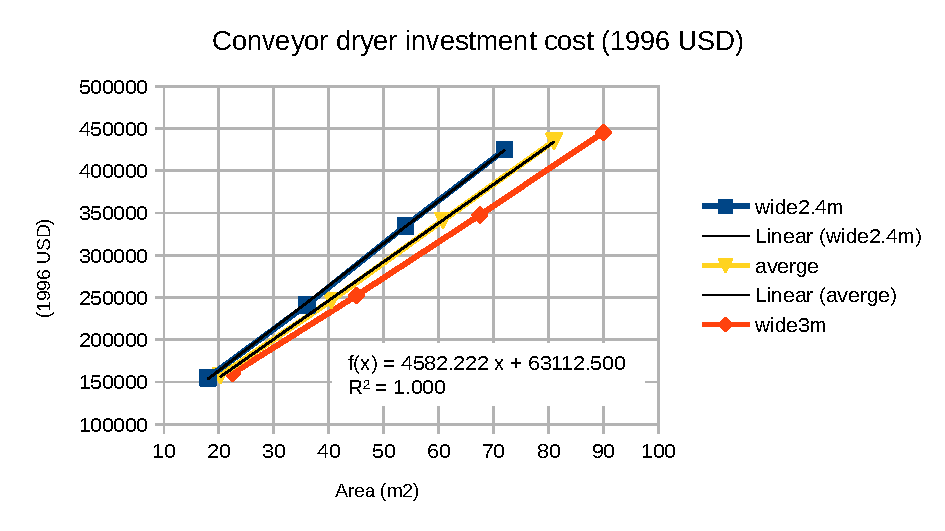
\includegraphics[width=0.6\linewidth]{converyor_dryer_investment_cost} 
%	\caption{Estimated investment costs for conveyor dryer unit.}
%	\label{fig:converyor_dryer_investment_cost2}
%\end{figure}

\section{Use of recovered nutirents as fertilizers}
\subsection{Struvite}
Some references can be found in Fig. \ref{fig:struvite_refs}

\begin{figure}[H]
	\centering
	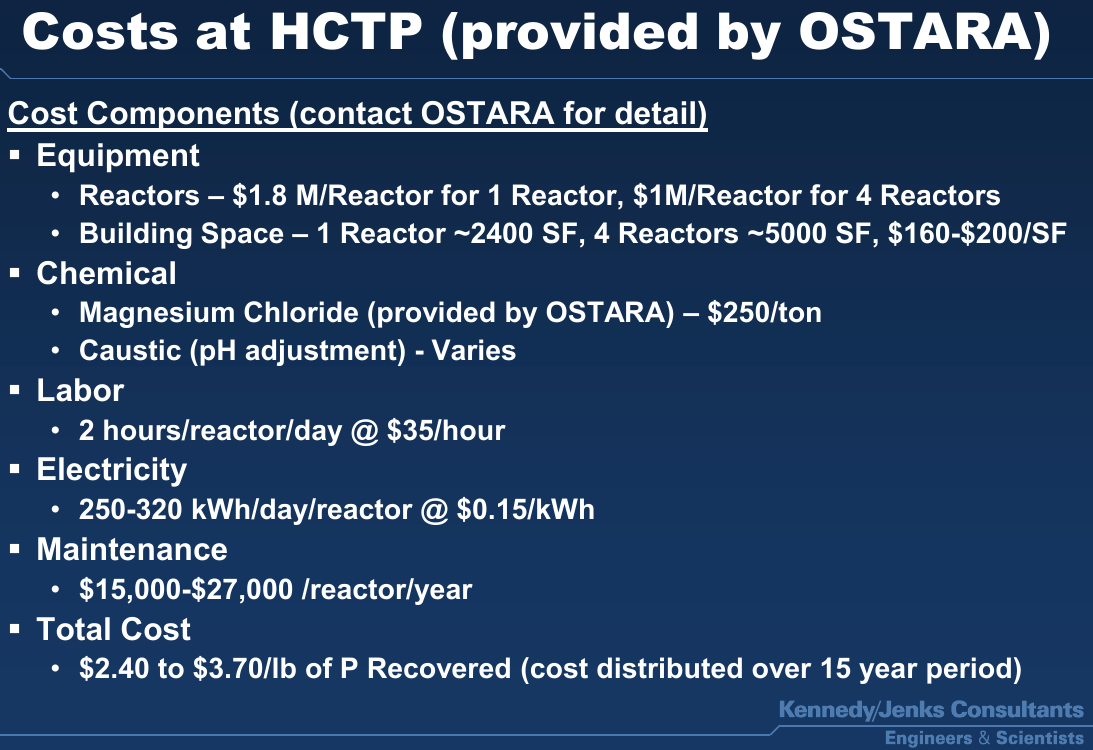
\includegraphics[width=0.6\linewidth]{ostara_costs} 
	\caption{References to evaluate the use of struvite pas fertilizer.}
	\label{fig:struvite_refs}
\end{figure}


\section{Indicators}
\subsection{Mid-point and end--point indicators}
When possible end-point indicators will be used to measure the final effect of the adoption of a particular technology, i.g. the harmful algal blooms develop as consequence of nutrient disposal on water bodies. However this is not possible in all cases, being make use of mid-point indicators. These indicators measure the direct impact of the process evaluated on the socioeconomic or environmental context, instead of the final consequence derived of these impact, i.g. the CO\textsubscript{2} emissions avoided rather than the global temperature increase avoided as consequence of the presence of this amount of carbon dioxide in the atmosphere.

\subsection{Metrics}
To measure the contribution to the sustainability and to be able to compare different technologies and scenarios, different indicators have been considered as measure units. With the aim to provide the most complete vision of the impact of the different alternatives development, three perspectives are considered: contribution to environmental sustainability, economic return, and social development. To give a balance measurement, the evaluation method includes indicators in each if these areas. Both total and specific measures are proposed to report both the total measure of each parameter, and the measure of the impact independently of the scale of the facility, allowing the comparison between different installations \cite{IChemE_sust_metrics}.

The boundaries considered to measure the impact of the implementation of the proposed processed involves from the waste stored in the facilities to its final disposal.


HISTORICAL TREND OF THE INDICATORS TO SHOW HOW THE ALREADY IMPLAMENTED FACILIES WORKS?

\subsubsection{Environmental indicators}
\paragraph{Energy usage}
\begin{align} 
& \text{Total net energy usage} \ \left(\frac{\text{kJ}}{\text{year}}\right) = \text{Energy used} - \text{Energy produced} \\
& \text{Specific net energy usage} \ \left(\frac{\text{kJ}}{\text{kg}_{\text{waste}}}\right) = \frac{\text{Energy used} - \text{Energy produced}}{\text{Waste processed}}
\end{align}

\paragraph{Water usage}
\begin{align} 
& \text{Total net water usage} \ \left(\frac{\text{kg}}{\text{year}}\right) = \text{Water used} - \text{Water recycled internally} \\
& \text{Specific net water usage} \ \left(\frac{\text{kg}}{\text{kg}_{\text{waste}}}\right) = \frac{\text{Water used} - \text{Energy produced}}{\text{Waste processed}}
\end{align}

\paragraph{Atmospheric acidification burden}
Mainly due to ammonia emissions.
\begin{align} 
& \text{Total atmospheric acidification burden} \ \left(\frac{\text{kg SO\textsubscript{2} equivalent}}{\text{year}}\right) = \sum_{n} \text{Mass flow}_{n} \cdot PFacid_{n} \\
& \text{Specific atmospheric acidification burden} \ \left(\frac{\text{kg SO\textsubscript{2} equivalent}}{\text{kg}_{\text{waste}}}\right) = \frac{\sum_{n} \text{Mass flow}_{n} \cdot PFacid_{n}}{\text{Waste processed}}
\end{align}

where $PFacid_{n}$ is the atmospheric acidification potency factor of substance $n$, reported in \cite{IChemE_sust_metrics}.

\paragraph{Global warming burden}
Mainly due to potential CO\textsubscript{2} amd CH\textsubscript{4} emissions.
\begin{align} 
& \text{Total global warming burden} \ \left(\frac{\text{kg CO\textsubscript{2} equivalent}}{\text{year}}\right) = \sum_{n} \text{Mass flow}_{n} \cdot PFwarm_{n} \\
& \text{Specific atmospheric acidification burden} \ \left(\frac{\text{kg CO\textsubscript{2} equivalent}}{\text{kg}_{\text{waste}}}\right) = \frac{\sum_{n} \text{Mass flow}_{n} \cdot PFwarm_{n}}{\text{Waste processed}}
\end{align}

where $PFwarm_{n}$ is the global warming potency factor of substance $n$, reported in \cite{IChemE_sust_metrics}.

\paragraph{Natural gas equivalent}
\begin{align} 
& \text{Total global warming burden} \ \left(\frac{\text{m\textsuperscript{3} nat. gas}}{\text{year}}\right) = \text{Total global warming burden} \cdot \frac{\text {Mass CO\textsubscript{2} generated}}{\text{Volume nat. gas}}
\end{align}

\paragraph{Ecotoxicity to aquatic life}
Mainly due to ammonia emissions.
\begin{align} 
& \text{Ecotoxicity to aquatic life} \ \left(\frac{\text{kg formaldehyde equivalent}}{\text{year}}\right) = \sum_{n} \text{Mass flow}_{n} \cdot PFeco_{n} \\
& \text{Specific ecotoxicity to aquatic life} \ \left(\frac{\text{kg formaldehyde equivalent}}{\text{kg}_{\text{waste}}}\right) = \frac{\sum_{n} \text{Mass flow}_{n} \cdot PFeco_{n}}{\text{Waste processed}}
\end{align}

where $PFeco_{n}$ is the ecotoxicity to aquatic life potency factor of substance $n$, reported in \cite{IChemE_sust_metrics}.

\paragraph{Eutrophication}
The excess of nutient in water bodies can develop the exponential growht of algae and cyanobacterias, causing harmful algal blooms (HABs). The harmful affects of HABs in the environment are, among others \cite{Morelli}:
\begin{itemize}
	\item Species shifts
	\item Depletion of oxygen due to algal decay
	\item Nuisance algae that affect other organisms
	\item Production of cyanotoxins that are harmful for aquatic life, wildlife and humans
\end{itemize}

The process for the development of HABs is shown in Fig. \ref{fig:HABs}

\begin{figure}[H]
	\centering
	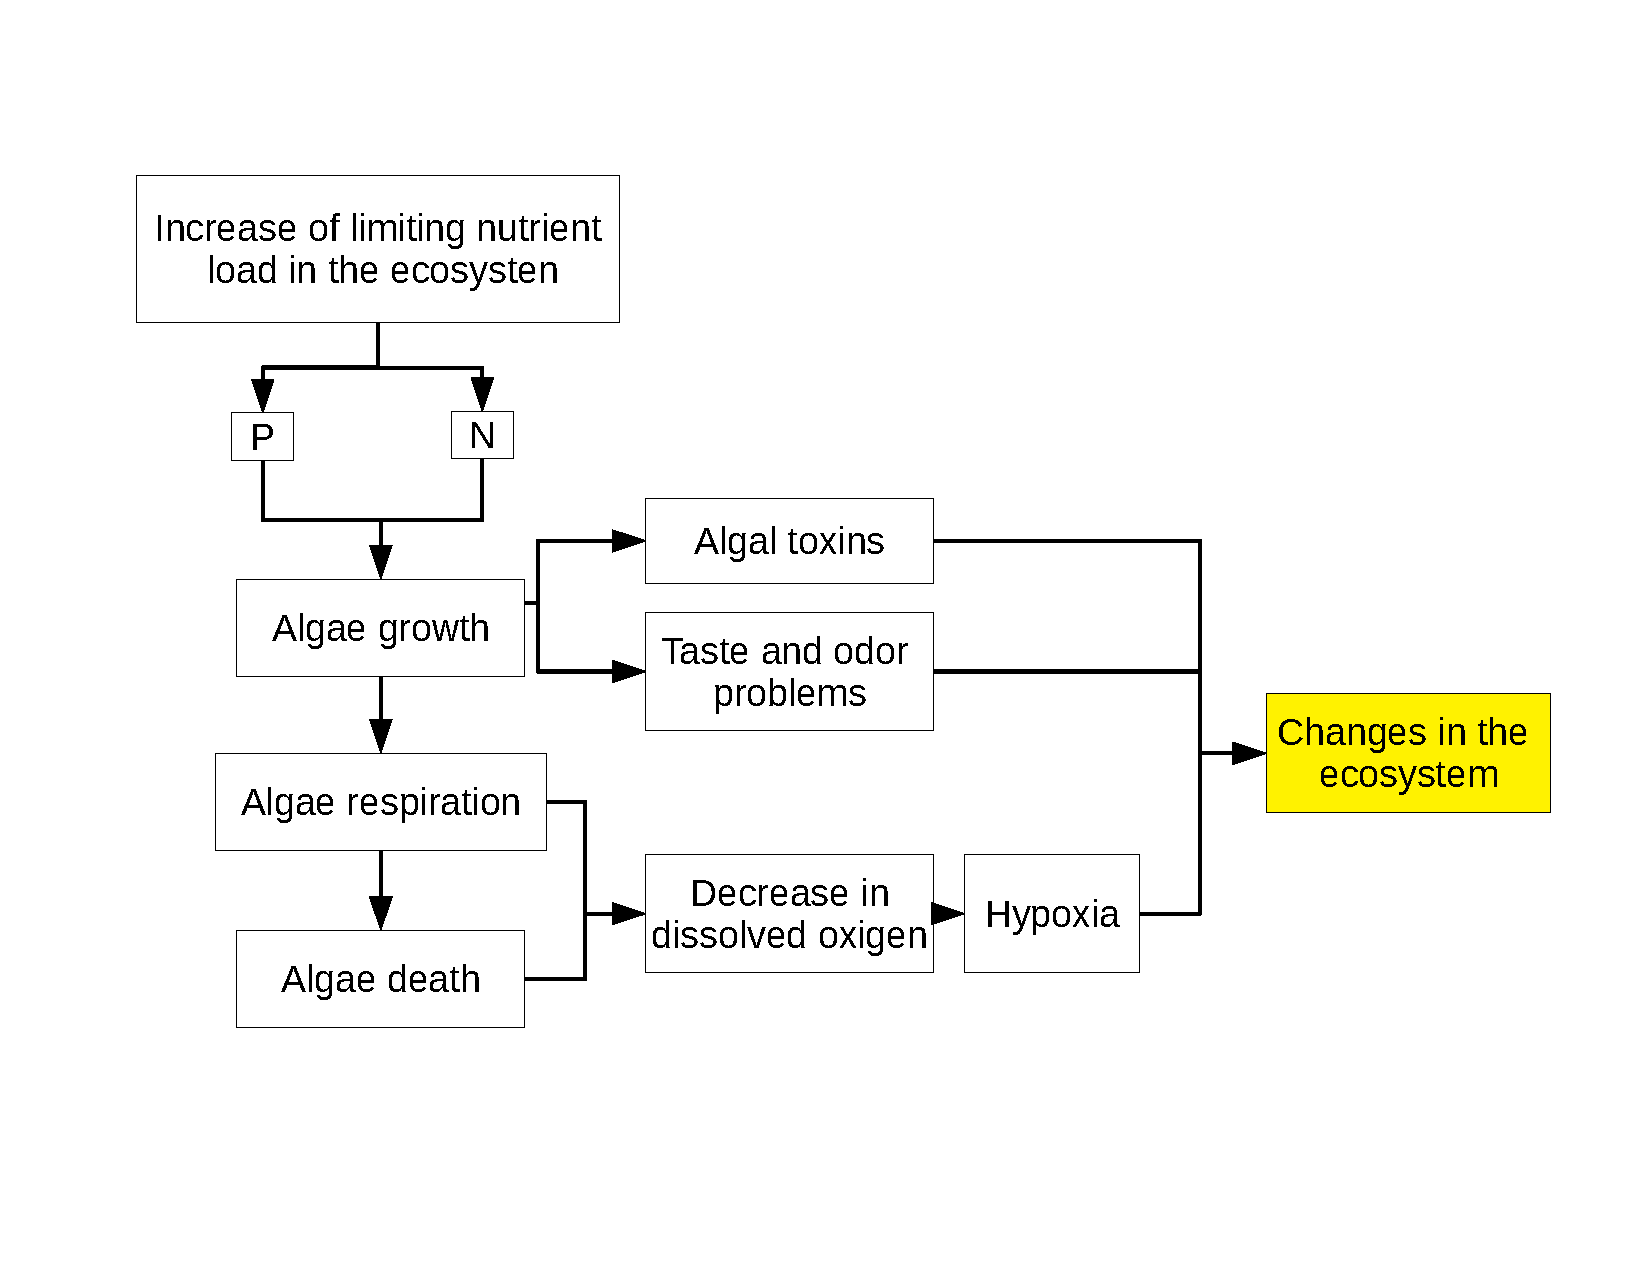
\includegraphics[width=0.6\linewidth, trim={2cm 4cm 1cm 2.5cm},clip]{HABs} 
	\caption{HABs development process.}
	\label{fig:HABs}
\end{figure}


Finally, the changes in the ecosystem result in environmental issues and economic losses due to both remediation precesses that must be applied and recreational and economic activities as fisheries that are interrupted.
Current models combine marine and freashwater environments as singles impact, as the indicators shown in Eqs. \ref{eq:eutrophcation_total} and \ref{eq:eutrophcation_specific}, or assume simplifications as P is the limitng nutrient in freshwater boides while N is the limiting nutrient in marine waters.

As characterizing factor of the impact of the P emission we proposed combine the threat due to the residence time of phosphorus in a particular area with the phosphorus concentration in that area to catch the spatialy effect in the eutrophication risk:
% and if the area is of special interest:
\begin{enumerate}
	\item Determine threat due to the residence time of phosphorus in a particular area using fate factor (FF) as measure.
	\item Determine phosphorus concentration on the area.
%	\item Determine if the area is of special interest.
	\item Combine the previous elements.
\end{enumerate}

To estimate the final effect over the freshwater ecosystem, a correlation between the HABs development and the presence of phosphorus over the geographical area studied has been developed to obtain a HABs developing probability indicator. Therefore, relating the characterizing factor calculated previously with HABs developing probability indicator we estimate the eutrophication risk of the emssions of a particular plant over a particular area. Linearity of the dose-response relationship: as other eutrophication indicators developed, a linear dose-response relationship is assumed \cite{IChemE_sust_metrics, ReCiPe_2016}.

The probability of HABs developmet is computed. A threshold that can not be exceeded is set.Additionally, it is considered if the land is under special protection, imposing a more restrictive threshold to the emissions of P,

%We are assuming the following considerations:
%
%\begin{itemize}
%	\item Linearity of the dose-response relationship: as other eutrophication indicators developed, a linear dose-response relationship is assumed \cite{IChemE_sust_metrics, ReCiPe_2016}.

%\begin{align} 
%& \text{Eutrophication} \ \left(\frac{\text{kg phosphate equivalent}}{\text{year}}\right) = \sum_{n} \text{Mass flow}_{n} \cdot PFeutro_{n} \label{eq:eutrophcation_total} \\
%& \text{Specific eutrophication} \ \left(\frac{\text{kg formaldehyde equivalent}}{\text{kg}_{\text{waste}}}\right) = \frac{\sum_{n} \text{Mass flow}_{n} \cdot PFeutro_{n}}{\text{Waste processed}} \label{eq:eutrophcation_specific}
%\end{align}
%
%where $PFeutro_{n}$ is the eutrophication potency factor of substance $n$, reported in \cite{IChemE_sust_metrics}.

\paragraph{HABs indicator}
As indicators for the incidence of HABs along the geography of the U.S., data from the National Aquatic Resource Surveys has been using, particularly those regarding the measurements made in the National Lake Assessment 2012 \cite{NLA2012QAPP}. The indicators selected were the concentration chlorophyll-a (Chl\emph{a}), since cyanobacteria only posses this kind of chlorophyll, and the content of microcystin. The idea behind the use two indicators is that the use of chlorophyll-a can be used to detemrinae the presence of both toxic and non-toxic blooms, whereas the use of microcystin is used to determine the toxic algal blooms. The metric selected for the evaluation of chlorophyll-a concentrations is the Carlson Trophic State Index \cite{CarlsonTSI}, which provide a ranking of the trophic state of the lakes, being a biological indicator aproved by the U.S. Environmental Protection Agency for the 2012 National Lakes assessment \cite{NLA2012QAPP}. As it is reported in the "National Lakes Assessment 2012: Technical Report" \cite{NLA2012techrep}, trophic is defined as of or relating to nutrition. Therefore, an eutrophic lake has high nutrients concentrations, associated with high algal and/or macrophyte plant growth, while an oligotrophic water body is characterized by low nutrient concentrations and low plant growth, being the mesotrophic state between the eutrophic and oligotrophic states. The Trophic State Classification is the same used by the U.S. EPA in the National Lakes Assessment 2012 \cite{NLA2012techrep}, shown in Table \cite{table:TSIclassification}.

\begin{table}[H] 
	\begin{adjustwidth}{}{}
		\centering
		\caption{Trophic State Classification \cite{NLA2012techrep}} \label{table:TSIclassification}
		\begin{tabular}{c c c c c}
			\toprule
			Analyte & Oligotrophic & Mesotrophic & Eutrophic & Hypereutrophic	\\ \midrule
			Chlorophyll-a ($\mu g$/L) & $\leq 2$ &  $>2 \text{and} \leq 7$ & $>7 \text{and} \leq 30$ & $>30$ \\ 
			\bottomrule 
		\end{tabular}
	\end{adjustwidth}
\end{table}


\paragraph{Impacts on protected areas}

\paragraph{Land impact (reduction of the fertility)}

\subsubsection{Economic indicators}
\paragraph{Yearly profit}
\paragraph{Net present value}

%The thermodynamic model also includes the mass balance to all components, defined by Eq. \ref{eq:balance2}.
%\begin{align} \label{eq:balance2}
%& \text{Total carbonates} = \left[  H_{2}CO_{3}\right] + \left[ HCO_{3}^{-}\right] + \left[ CO_{3}^{2-}\right]
%\end{align}


%\subsubsection{Initial solid species supersaturation indexes} \label{precipitates}
%%In a similar way than for aqueous species equilibrium, the thermodynamic equilibrium for the solids species are calculated, and 
%After determining the species distribution for the aqueous systems, the initial supersaturation indexes for initial conditions are computed, determining the formed precipitates. The solids species considered in this study are shown in Table \ref{table:solids_species}:
%\begin{table}[H] 
%	\begin{adjustwidth}{}{}
%		\centering
%		\caption{Solids species considered.} \label{table:solids_species}
%		\begin{tabular}{c c c c}
%			\toprule
%			Name	& Chemical system &${pK}_{{sp}}$	&Source	\\ \midrule
%			Struvite	& $MgNH_{4}PO_{4} \cdot 6H_{2}O \leftrightarrow Mg^{2+} + NH_{4}^{+} + PO_{4}^{3-}$ &13.26 &\cite{Ohlinger} 	\\ 
%			K-struvite	& $MgKPO_{4} \cdot 6H_{2}O \leftrightarrow Mg^{2+} + K^{+} + PO_{4}^{3-}$ & 10.6 & \cite{TaylorAW}  	\\ 
%			Hydroxyapatite	& $Ca_{5} \left( PO_{4} \right)_{3}OH \leftrightarrow 5Ca^{2+} + 3PO_{4}^{3-}+OH^{-}$ &44.33 &\cite{Brezonik}  \\ 
%			Calcium carbonate	& $CaCO_{3} \leftrightarrow Ca^{2+} + CO_{3}^{2-}$ &8.48	&\cite{Morse} \\ 
%			Tricalcium phosphate	& $Ca_{3} \left( PO_{4} \right)_{2} \leftrightarrow 3Ca^{2+} + 2PO_{4}^{3-}$ &25.50 &\cite{Fowler} 	\\
%			Dicalcium phosphate	& $CaHPO_{4} \leftrightarrow Ca^{2+} + HPO_{4}^{2-}$ &6.57	&\cite{Gregory} 	\\
%			Calcium hydroxide	& $Ca \left( OH \right)_{2} \leftrightarrow Ca^{2+} + 2OH^{-}$ &5.19  &\cite{Skoog}  \\
%			Magnesium hydroxide	& $Mg(OH)_{2} \leftrightarrow Mg^{2+} + 2OH^{-}$&11.15  &\cite{Skoog} 	\\  \bottomrule 
%		\end{tabular}
%	\end{adjustwidth}
%\end{table}

%The supersaturation index is computed through the thermodynamic equilibrium, defined by the Eq. \ref{eq:Omega_i} for all the components described above:
%\begin{align} \label{eq:Omega_i}
%\Omega_{i}= \frac{ \prod \left\{ Products \right\}_{i} }{ K_{sp_{i}}  }
%\end{align}
%Where $pK_{sp}$ values are collected in Table \ref{table:solids_species}. Note that:
%\begin{align*}
%& \Omega_{i} > 1, \qquad \text{element} \ i \ \text{precipitates} \\
%& \Omega_{i} = 1, \qquad \text{element} \ i \ \text{reachs saturation} \\
%& \Omega_{i} < 1, \qquad \text{element} \ i \ \text{not precipitate} \\
%\end{align*}



%\begin{figure}[H]	
%	\begin{subfigure}[t]{0.5\linewidth}
%		\includegraphics[width=\linewidth]{plotHAP_Ca} 
%		\caption{Evolution of hydroxyapatite formation along $Ca^{2+}/PO_{4}^{3-}$ molar ratio values considering 50 different composition data sets.}
%		\label{fig:estimation_Ca_HAP}
%	\end{subfigure}
%	\qquad
%	\begin{subfigure}[t]{0.5\linewidth}
%		\includegraphics[width=\linewidth]{plotCaCO3_Ca}
%		\caption{Evolution of calcium carbonate formation along $Ca^{2+}/PO_{4}^{3-}$ molar ratio values considering 50 different composition data sets.}
%		\label{fig:estimation_Ca_CaCO3}
%	\end{subfigure}
%	
%	\caption{Evolution of calcium precipitates formation along $Ca^{2+}/PO_{4}^{3-}$ molar ratio values considering 50 different composition data sets.}
%	\label{fig:estimation_Ca_ca}
%\end{figure}



\bibliographystyle{ieeetr}
\bibliography{references}

\end{document}